\documentclass[11pt]{book}
\usepackage{amsmath}
\usepackage[russian]{babel}
\usepackage{color}
\usepackage{fullpage}
\usepackage[utf8]{inputenc}
\usepackage{graphicx}
\usepackage{listings}

% for nice symbols
\usepackage{amssymb}
\usepackage{textcomp}
\usepackage{wasysym}
\usepackage{marvosym}

\title{
\small{\textleaf}
\huge{\textleaf}
\huge{\quad}
\large{Сказ о том, чем компилятор от интерпретатора отличается :)}
\huge{\quad}
\huge{\textleaf}
\small{\textleaf}
}
\author{
\small{\textborn} \ 
\small{\APLstar} \ 
\huge{\textborn} \ 
\huge{\APLstar} \ 
\Huge{$\bigstar$} \ 
\huge{\APLstar} \ 
\huge{\textborn} \ 
\small{\APLstar} \ 
\small{\textborn}
\\
\Large (в вольном изложении братца)
\\
\huge{\Bicycle}
}
\date{май 2014}

\begin{document}

\maketitle
\pagebreak

\section*{Што это такое}
Программирование сильно смахивает на героическую борьбу человека с компьютером.
Человек пишет программу. Он пишет её на странном, нелогичном языке, с трудом выражая
свои мысли. Язык больше мешает, чем помогает: нужной функции нет, зато есть
куча каких-то дурацких никому не нужных штук.
\\ \\
Вот человек написал программу. Посидел, порассматривал своё кривоватое детище.
С виду --- странная смесь английских слов и бессмысленных крикозябликов.
Но цепкие глаза программиста смотрят сквозь буквы, въедаются
в неуловимую суть. Наконец человек устаёт пыриться в экран и отдаёт программу
на суд компьютера. Начинается долгое, утомительное противостояние: человек
то букву добавит, то две уберёт, то вообще начинает удалять текст большими кусками.
\\ \\
И вот наступил великий момент: программа запустилась. На чёрном фоне
высветились белые буквы ``Segmentation fault''.
\\ \\
Что я хочу сказать этой болтовнёй, так это то, что языки программирования малость не идеальны. :D
Я хотела рассказать тебе, что я о них знаю, что меня вдохновляет
и позволяет худо-бедно продираться через сотни костылей и заведомую плохость результата.
\\ \\
План у меня примерно такой.
Я начну с того, что такое машинный язык, потому что без понимания этого всё остальное --- отвязанная от жизни болтовня.
Потом я расскажу, как от машинного языка можно перейти к языкам высокого уровня.
Потом попытаюсь упомянуть ключевые вещи в языках программирования.
Ну и главное (и самое нудное) --- детсадовский, но вполне рабочий пример.
\\ \\
Эта бумажка не поможет тебе узнать всё и сразу.
Скорее она предназначена, чтобы научить тебя искать в правильном направлении и ничего не бояться.
(Думаю, ты умеешь это лучше меня, но специфика у тебя вроде чуток другая.)
По крайней мере, я отчаянно пыталась показать, что нет магии, что в каждой мелочи можно докопаться до истоков,
всё понять своей головой.
Мне самой пришлось много гуглить и читать мануалы, чтобы объяснить некоторые куски примера.
\\ \\
Пример я привожу не просто на словах: это код реальной программы, и программа прилагается.
Было б классно, если бы ты поковыряла эту программу, попробовала поменять там разные штуки
(особенно в тех местах, на которых я подолгу останавливаюсь).
Книжки, которые я упоминаю, хотя бы просто открой: пролистать оглавление --- уже большое дело.
\\ \\
Есть много книжек, которые стоит прочитать.
Не для того, чтобы стать очень умной --- это мелкий побочый эффект.
Просто программирование без идеи --- на редкость нудное дело, а идея как фонарь --- то потухнет, то погаснет.
Книжки, то есть мысли других людей, не дадут твоей идее погаснуть.
Я их люблю за это, а умность --- хоть бы её и совсем не было.
\\ \\
Из совсем уж классных книжек:
Petzold, ``Code'' (про устройство компьютера);
Tanenbaum (он много про что написал: архитектура компьютеров, компьютерные сети);
SICP (Structure and Interpretation of Computer Program, я лично читала, но собираюсь, хорошие люди советуют);
Jacobs, Grune: ``Parsing Techniques. A Practical Guide'', 2nd edition (моя лично горячо любимая книжка про синтаксический анализ);
Kline: ``Mathematics: the Loss of Certainty'' (про историю и смысл математики).
И другие...

\tableofcontents

\chapter{Как устроен компьютер}
Допустим, ты решишь написать программу, которая умножает два числа,
введённых пользователем с клавиатуры, а потом исполнить её на компьютере.
Скорее всего, ты будешь действовать примерно так:
\begin{enumerate}
\item включишь компьютер
\item запустишь Microsoft Visual Studio
\item создашь новый проект типа Console Application
\item добавишь в проект файл main.cpp
\item в файле main.cpp наберёшь текст:
\item{
\begin{verbatim}
    #include <iostream>

    int main ()
    {
        int a;
        int b;

        std::cout << "Enter a:" << std::endl;
        std::cin >> a;
        std::cout << "Enter b:" << std::endl;
        std::cin >> b;
        std::cout << "a * b = " << a * b << std::endl;

        return 0;
    }
\end{verbatim}}
\item Нажмёшь на зелёный треугольник: выскочит чёрное окошко
    с приглашением ввести первое число.
\end{enumerate}
Потом ты задумаешься: а что собственно происходит при
нажатии на зелёный треугольник? Ответ на этот вопрос
примерно такой:
\begin{enumerate}
\item Компиляция.
\\
    Visual Studio запускает встроенный в неё компилятор C++ и передаёт
    ему в качестве аргумента файл main.cpp. Компилятор преобразует код
    на языке C++ в файле main.cpp в код на машинном языке, и сохраняет
    его в новый файл (например main.o). Такой файл с машинными кодами
    называется \emph{объектным} файлом (отсюда и расширение .o).
\item Линковка.
\\
    Каждый .cpp файл преобразуется компилятором в отдельный объектный файл.
    Сами по себе объектные файлы не самодостаточные:
    в одном из них могут использоваться функции, определённые в другом.
    Поэтому объектные файлы нужно объединить в один, и настроить связи
    между ними. Этим занимается линкер.
\\
    Кстати, наш файл main.o тоже не самодостаточный, он использует
    библиотечные функции для ввода-вывода.
\item Исполнение.
\\
    После линковки получается один большой \emph{исполняемый} файл (main.exe).
    Чтобы машинный код в файле main.exe начал исполняться на процессоре,
    нужно во-первых загрузить его в оперативную память, а во-вторых
    указать процессору, с какого адреса в памяти начинать исполнять инструкции
    (то есть передать управление на начало этого кода). Этим занимается загрузчик.
\end{enumerate}
В этом объяснении многое остаётся непонятным. Наверное,
самое непонятное, это ``машинный код''. Чем он так сильно отличается
от другого кода, что вдруг становится понятным процессору?
Другая странность --- это тайная связь оперативной памяти и процессора.
Почему-то, чтобы процессор начал исполнять машинный код, надо загрузить
этот код в оперативную память. А где он был до этого? И что значит
``указать процессору, с какого адреса в памяти начинать исполнять
инструкции''?
\\ \\
Чтобы это понять, надо представлять, как устроен компьютер. В общем,
есть четыре основных компонента, без которых ну никак:
\begin{enumerate}
\item процессор
\item память
\item устройство ввода
\item устройство вывода
\end{enumerate}
У процессора две главных функции: выполнять арифметико-логические операции
(складывать, умножать, сравнивать и т.д.), и задавать темп работы
(отсчитывать такты). Память, нужна чтобы хранить в ней что-то, иначе всё, что насчитал
процессор, потеряется. Ну и наконец, без устройств ввода/вывода с компьютером вообще ничего нельзя
сделать.
\\ \\
Такое объяснение не противоречит здравому смыслу, но и только. Оно слишком
общее, чтобы понять, что такое машинный код и как исполняются программы.
Кроме того, непонятно, почему компьютер должен быть
устроен именно так: то-ли по законам природы, то-ли по чудовищной случайности.
Поэтому щас я попытаюсь пошагово построить компьютер: начну с
необходимого минимума и буду постепенно добавлять элементы,
которые не сделаешь на основе тех, что уже есть.

\section{Физическая основа}
Компьютер придумали для автоматизации вычислений. Автоматизация
вычислений произошла по четырём причинам:
\begin{enumerate}
\item люди считают медленно
\item люди допускают ошибки
\item людям лень считать
\item люди невероятно умные
\end{enumerate}
Поэтому естественная для человека мысль --- использовать какой-то
физический процесс для своих целей. Можно сплавлять брёвна вниз по реке.
Можно построить водяную или ветряную мельницу. Можно сделать песочные часы.
\\ \\
В основе компьютера тоже должен лежать какой-то физический процесс,
и сейчас это электричество. Но надо понимать, что чисто теоретически вместо
электричества может быть что угодно (и было: первые компьютеры были механические,
а в последнее время некоторые пытаются построить компьютер на основе какого-то
хитрого вида плесени).
\\ \\
С другой стороны, надо понимать, что электричество в компьютерах не случайно:
оно во многом \emph{позволило} сделать компьютер. Механический компьютер
той же сложности, что твой ноут, был бы невменяемого размера.
Все процессы шли бы в нём крайне медленно (пока шестерёнки с одного
конца докрутятся до другого). Кроме того, детали в этом компе ломались бы так часто,
что комп был бы всё время сломан.

\subsection{Электрические схемы и логика}
Начнём с простой схемы:
\\
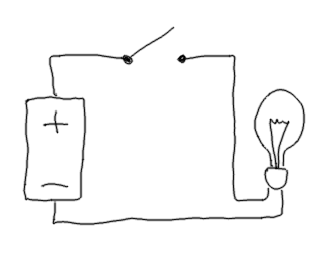
\includegraphics[height=1in]{pic/2.png}
\\
В этой цепи немного элементов: лампочка, батарея, ключ. Если ключ разомкнут,
ток не идёт, и лампочка не горит. Если ключ замкнут, ток идёт, и лампочка горит.
Кстати, лампочка нас интересует только как индикатор, есть ток или нет.
В целом зависимость ``лампочка - ключ'' можно охарактеризовать таблицей:
\\
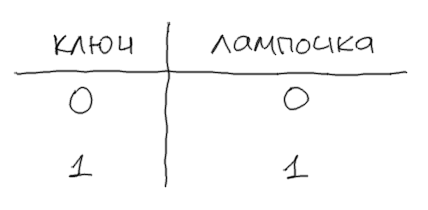
\includegraphics[height=1in]{pic/3.png}
\\
Таблицы такого рода, задающие зависимость истинности/ложности одних переменных
от истинности/ложности других переменных, называются \emph{таблицами истинности} или \emph{таблицами логики}.
Добавим ещё один ключ в схему (последовательно):
\\
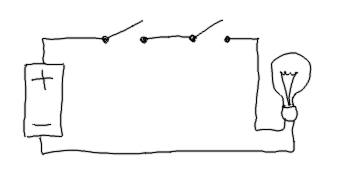
\includegraphics[height=1in]{pic/4.png}
\\
Теперь лампочка зависит от двух ключей: она горит, только если первый
\emph{и} второй ключ замкнут. Вот соответствующая таблица логики:
\\
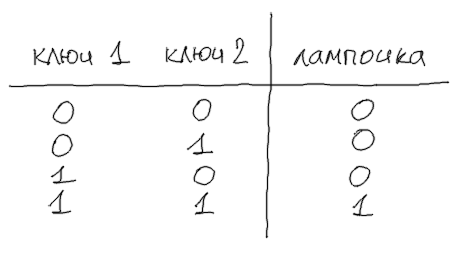
\includegraphics[height=1.5in]{pic/5.png}
\\
Если бы мы добавили второй ключ параллельно, схема бы получилась такой:
\\
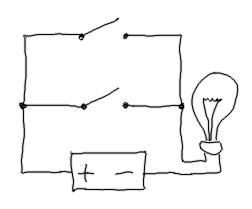
\includegraphics[height=1.5in]{pic/6.png}
\\
В этой схеме лампочка горит, только если первый \emph{или} второй ключ замкнут.
Вот её таблица логики:
\\
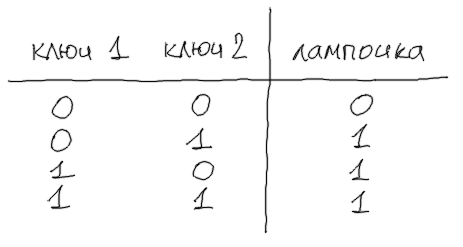
\includegraphics[height=1.5in]{pic/7.png}
\\
Мы получили две интересных схемы: первая отражает логическое \emph{и} (AND), вторая ---
логическое \emph{или} (OR). На основе этих схем можно собирать другие, более сложные.
Например, есть у тебя условие: ``если я сдам лабу или будет солнечно,
то я пойду гулять''. Это условие описывается схемой OR:
\\
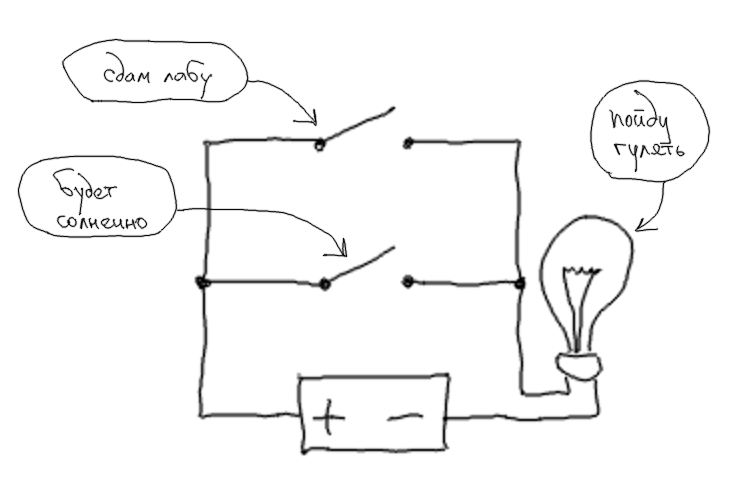
\includegraphics[height=2in]{pic/8.png}
\\
Преподаватель, которому ты собралась сдавать лабу, знает, что если у него
будет хорошее настроение, то ты сдашь лабу. Его настроение зависит от двух вещей:
во-первых, будет ли солнечно, а во вторых, успеет ли он пообедать.
Он может описать это с помощью схемы AND:
\\
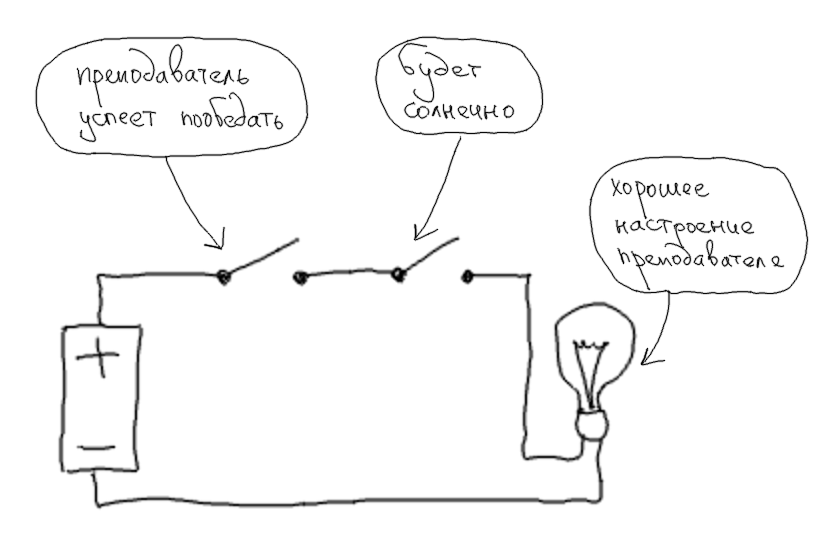
\includegraphics[height=2in]{pic/9.png}
\\
Допустим, преподаватель хочет узнать, пойдёшь ли ты завтра гулять, но не очень
хорошо разбирается в хитросплетениях твоей логики. Зато у него есть твоя схема.
Он берёт её и пытается присобачить к ней свою. Логически это очень просто:
нужно связать выход ``хорошее настроение'' со входом ``сдам лабу'': если на выходе
``хорошее настроение'' есть ток, ключ ``сдам лабу'' замкнут, если тока нет --
разомкнут:
\\
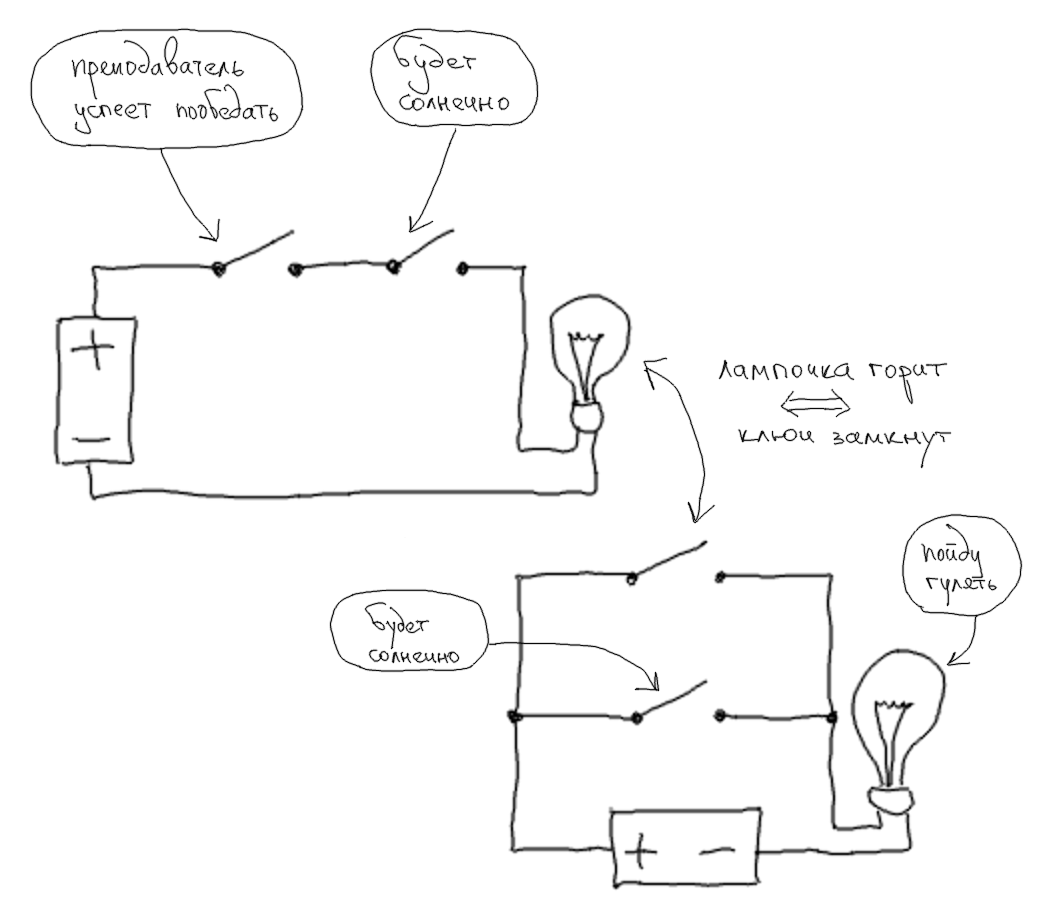
\includegraphics[height=3.5in]{pic/10.png}
\\
Поначалу можно вручную замыкать и размыкать ключ, но это быстро надоест
(особенно когда схема станет большой). Нужно что-то, что само замыкало и
размыкало бы ключ в зависимости от тока. Одним из таких устройств является
реле:
\\
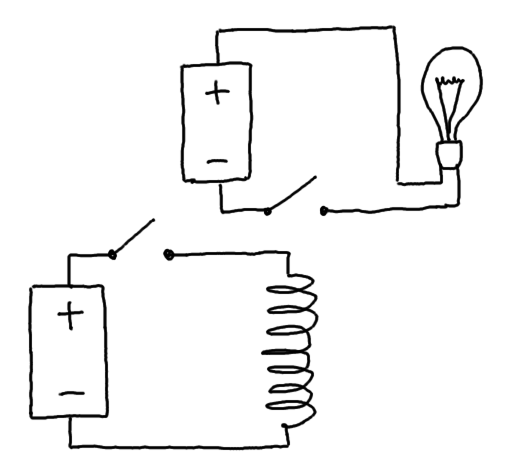
\includegraphics[height=2in]{pic/11.png}
\\
Если в первой цепи течёт ток, то катушка намагничивается и начинает притягивать
ключ во второй цепи. Ключ замыкается. Если в первой цепи ток пропадает, то катушка размагничивается,
перестаёт притягивать ключ и он размыкается. Реле позволяет связать вход
``сдам лабу'' с выходом ``хорошее настроение'':
\\
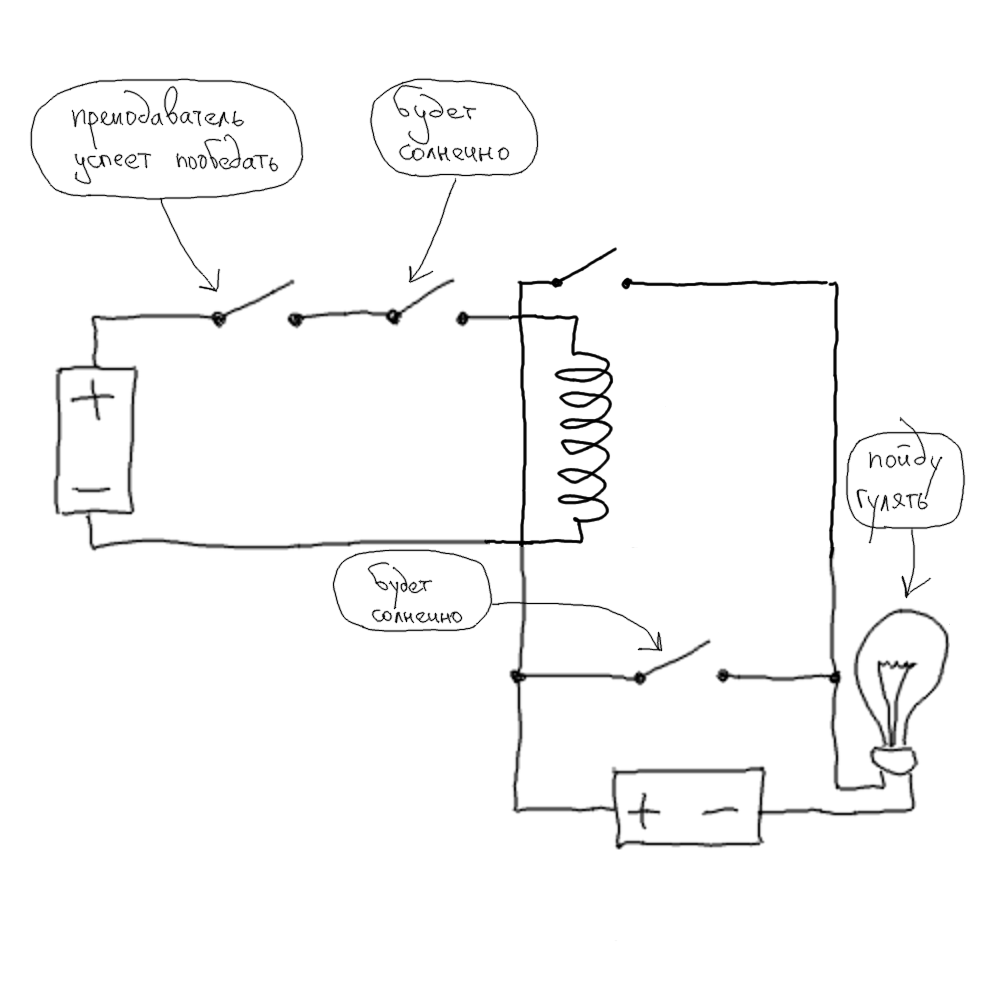
\includegraphics[height=3.5in]{pic/12.png}
\\
Конечно, эту конкретную схему можно упростить и выкинуть реле, просто встроив преподавательскую схему
в твою вместо ключа ``сдам лабу'':
\\
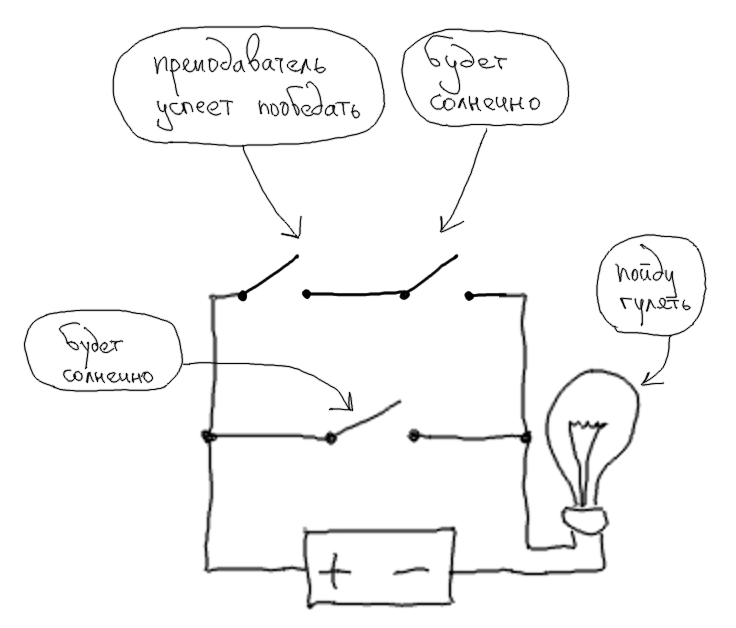
\includegraphics[height=3.5in]{pic/13.png}
\\
И даже ещё сильнее упростить:
\\
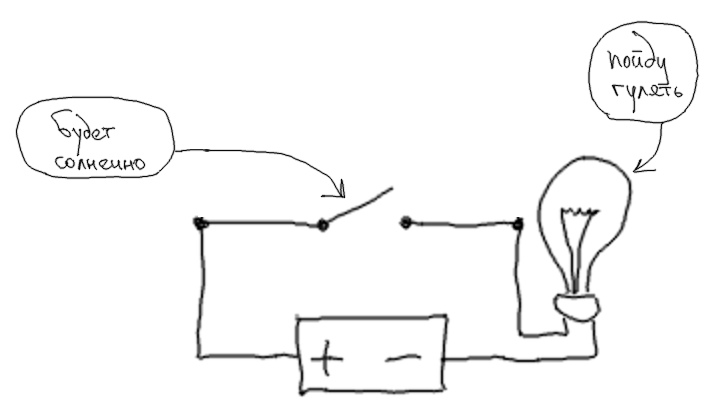
\includegraphics[height=2in]{pic/14.png}
\\
Но упростить не всегда возможно и никогда не поздно, и пусть этим занимаются разработчики микросхем.
Мне важно показать, что схему в принципе \emph{можно} собрать. Реле позволяет нам управлять входом схемы при помощи наличия/отсутствия тока,
а не при помощи замыкания/размыкания ключа. А наличие/отсутствие тока --- это как раз то,
что является выходом любой схемы. Поэтому можно сделать очень
важное предположение: что любой выход одной схемы можно соединить с любым входом другой
схемы. (Кстати, реле полезно не только для связывания разных схем, а ещё и просто как повторитель, для усиления слабого тока.
Именно для передачи сигнала на большие расстояния реле использовалось в телеграфных линиях.)
\\ \\
Реле --- не единственное устройство, способное замыкать и размыкать ключ
в зависимости от тока (но первое, которое применили в компьютерах). Сейчас
используются транзисторы, а до этого были вакуумные лампы.
\\ \\
Вот как выглядят схемы AND и OR с использованием реле:
\\
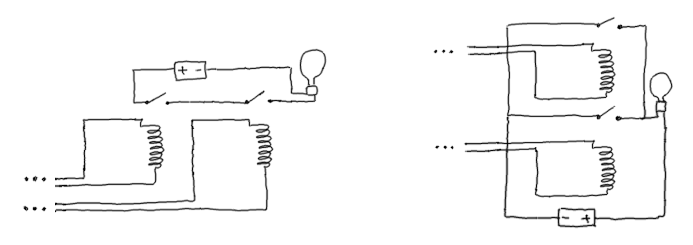
\includegraphics[height=2in]{pic/15.png}
\\
Строго говоря, это уже не схемы, а фрагменты схем. Но, с другой стороны, ``выход'' схемы ---
тоже не выход, а кусок цепи, по которому идёт или не идёт ток. Чтобы соединить выход
и фрагмент, нужно разомкнуть цепь в районе выхода и получившиеся два конца провода примотать
к концам провода, торчащим из фрагмента:
\\
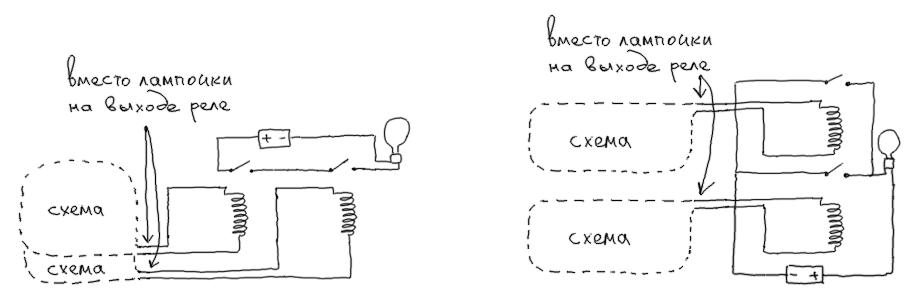
\includegraphics[height=2in]{pic/16.png}
\\
Дальше я всё буду называть схемой. Вот ещё одна важная схема, отражающая ``логическое \emph{не}'', NOT:
\\
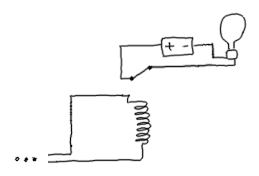
\includegraphics[height=1.5in]{pic/17.png}
\\
В предыдущих схемах реле повторяло сигнал, а здесь оно его инвертирует: если в первой цепи идёт ток, то во второй тока нет, и наоборот.
Поэтому схема называется \emph{инвертором}.
\\ \\
Оказывается, что вместе три эти простенькие схемы --- И, ИЛИ, НЕ --- обладают невероятной силой.
С помощью них можно собрать ЛЮБУЮ логическую схему! (И это ещё не всё: из схем И и НЕ можно
собрать схему ИЛИ, а из схем ИЛИ и НЕ можно собрать схему И. Есть вообще такие схемы И-НЕ и ИЛИ-НЕ,
что с помощью каждой из них (одной) можно собрать все остальные. Дальше по этой
теме читай про ``полные системы булевых функций''.)
\\ \\
Для этих трёх схем --- И, ИЛИ, НЕ --- я введу общепринятые обозначения:
\\ \\
Как видишь, входы и выходы обозначаются одинаково, в виде куска торчащего
провода. Я буду говорить ``подать ток на вход''. Понятно, что с точки зрения физики это
бред, потому что нельзя просто так взять и подать ток куда-то. Но (надеюсь) понятно,
что я имею в виду.
\\ \\
Почти всё дальнейшее построение компьютера сведётся к сборке более сложных схем
из этих трёх.

\subsection{Двоичная система счисления}
Я вот всё время говорю про логические схемы и булевые функции (что по сути одно и то же),
и даже собрала маленькую схему для определения, пойдёшь ли ты гулять. Более того, я собрала
несколько простых схем (И, ИЛИ, НЕ) и говорю, что с их помощью можно собрать
любую логическую схему. В смысле логических схем наще будущее явно обеспечено.
Но всё-таки, какая ИМЕННО от них польза?
\\ \\
Пока понятно только, что электричество удивительно хорошо для них подходит.
В электричестве есть два чётких состояния: есть ток, нет тока. И в логике
есть два элемента: правда, ложь. Если б мы захотели с помощью электричества моделировать
социальные анкеты (``да'', ``нет'', ``не знаю''), нам пришлось бы выдумывать, как обозначать
третий элемент (например, есть ток, но слабый). Тем более тяжело было бы
с десятичными цифрами.
\\ \\
А мы-то как раз с цифрами (вернее, с числами) работать и собрались, потому что
что это за компьютер, который даже два числа сложить не может. К счастью, нам не
придётся моделировать десять состояний (в отличие от тех, кто строил первые
компьютеры). Мы просто будем все вычисления внутри компьютера проводить над числами
в двоичном представлении.
\\ \\
Важное замечание: от того, что мы решили использовать в компьютере двоичные,
а не десятичные числа, С ТОЧКИ ЗРЕНИЯ ПОЛЬЗОВАТЕЛЯ НИЧЕГО НЕ МЕНЯЕТСЯ: число
это просто абстрактная идея, и не важно, в каком виде она выражена. Компьютер
будет делать ровно то же, что и с десятичными числами: решать такие же задачи
и выдавать такие же результаты. Потом, если угодно, можно сделать специальную приставку,
которая будет позволять вводить/выводить десятичные числа, и переводить их
для компьютера в двоичное представление.

\section{Сумматор}
Итак, компьютер нужен для автоматизации вычислений.
Поэтому первое, без чего не обойдётся ни один компьютер, это устройство
для сложения чисел. Попробуем собрать такое устройство --- сумматор.
\\ \\
Чтобы понять, как должен работать двоичный сумматор, надо
вспомнить, что делает человек, когда складывает двоичные числа.
Сложение происходит поразрядно и с переносом:

\begin{enumerate}
\item
   k = 1
\\
   перенос = 0
\\
   если одно число короче другого, дополнить его нулями в старших разрядах
\\
   N = число разрядов
\\
\item Определяем k-й разряд первого суммы и новый перенос по таблице:
\begin{verbatim}
   -------------------------------------------------------------------
   | k-й разряд    | k-й разряд    | перенос || k-й разряд | перенос |
   | первого числа | второго числа |         || суммы      | (новый) |
   |---------------|---------------|---------||------------|---------|
   |       0       |       0       |    0    ||     0      |    0    |
   |       0       |       0       |    1    ||     1      |    0    |
   |       0       |       1       |    0    ||     1      |    0    |
   |       0       |       1       |    1    ||     0      |    1    |
   |       1       |       0       |    0    ||     1      |    0    |
   |       1       |       0       |    1    ||     0      |    1    |
   |       1       |       1       |    0    ||     0      |    1    |
   |       1       |       1       |    1    ||     1      |    1    |
   -------------------------------------------------------------------
\end{verbatim}
\item k = k + 1
\item если k < N
\\
       перейти к шагу 2
\end{enumerate}


Видимо, главное в этом алгортме --- таблица, по которой определяются новый перенос
и k-й разряд суммы. Без этой таблицы не обойтись: в жизни мы принимаем как аксиому,
что 0+0=0, 0+1=1, 1+0=1, 1+1=0 и 1 в уме. В сумматор тоже придётся встроить эти
правила.
\\ \\
Итак, нам нужна схема, у которой три входа: k-й разряд первого слагаемого,
k-й разряд второго слагаемого и перенос, и два выхода: k-й разряд суммы и перенос
на (k + 1)-й разряд. Отстуствие тока на входе или выходе означает ноль,
наличие --- единицу. Внутри схема должна быть устроена так, чтобы зависимость
выходов от входов была такая же, как в таблице.
\\ \\
Это очень похоже на схемы И, ИЛИ, НЕ, только наша схема более сложная.
Чтобы слегка упростить схему, разобьём её на две полсхемы. Сделать это
можно так: вместо того, чтобы сразу пытаться сложить три входа
(k-й разряд первого числа, k-й разряд второго числа, перенос), будем
два раза складывать по два входа: сначала k-й разряд первого числа и k-й разряд второго числа,
а потом результат первого сложения и перенос.
\\ \\
Когда складываешь два входа, может возникнуть перенос (если оба входа равны 1).
Поэтому у каждой полсхемы будет два входа (для слагаемых) и два выхода
(для суммы и переноса):
\begin{verbatim}
   ----------------------------------------------------
   | 1-е слагаемое | 2-е слагаемое || сумма | перенос |
   |               |               ||       |         |
   |---------------|---------------||-------|---------|
   |       0       |       0       ||     0 |     0   |
   |       0       |       1       ||     1 |     0   |
   |       1       |       0       ||     1 |     0   |
   |       1       |       1       ||     0 |     1   |
   ----------------------------------------------------
\end{verbatim}
Чтобы собрать такую полсхему, снова разобьём её на две четвертьсхемы,
одна для суммы, а вторая для переноса:
\begin{verbatim}
   ------------------------------------------
   | 1-е слагаемое | 2-е слагаемое || сумма |
   |               |               ||       |
   |---------------|---------------||-------|
   |       0       |       0       ||     0 |
   |       0       |       1       ||     1 |
   |       1       |       0       ||     1 |
   |       1       |       1       ||     0 |
   ------------------------------------------
   --------------------------------------------
   | 1-е слагаемое | 2-е слагаемое || перенос |
   |               |               ||         |
   |---------------|---------------||---------|
   |       0       |       0       ||     0   |
   |       0       |       1       ||     0   |
   |       1       |       0       ||     0   |
   |       1       |       1       ||     1   |
   --------------------------------------------
\end{verbatim}

Четвертьсхема для переноса совсем простая --- это попросту схема И.
С суммой всё не так просто, но взяв две схемы ИЛИ, одну схему НЕ и одну схему И,
мы получим то, что надо:
\\ \\
Остаётся объединить входы четвертьсхем для суммы и переноса,
и полсхема для сложения двух входов готова:
\\ \\
Теперь пора связать полсхемы. У первой полсхемы два входа:
k-й разряд первого слагаемого и k-й разряд второго слагаемого.
У второй полсхемы первый вход --- это выход ``сумма'' первой полсхемы,
а второй вход --- перенос:
\\ \\
У нас остался один выход ``сумма'' --- как раз как надо. Но выходов ``перенос'' по прежнему два,
а нужен один. Из-за разбиения сложения на два этапа на каждом этапе получился свой перенос.
Но ведь в жизни всё равно, сразу три числа складывать, или сначала сложить два, а потом прибавить
третье --- результат один и тот же. Что-то тут не то! Если повнимательнее рассмотреть полученную нами схему
с тремя выходами, то её работа описывается такой таблицей логики:
\begin{verbatim}
   -------------------------------------------------------------------------------------
   | k-й разряд    | k-й разряд    | перенос || k-й разряд | 1-й перенос | 2-й перенос |
   | первого числа | второго числа |         || суммы      |             |             |
   |---------------|---------------|---------||------------|-------------|-------------|
   |       0       |       0       |    0    ||     0      |    0        |    0        |
   |       0       |       0       |    1    ||     1      |    0        |    0        |
   |       0       |       1       |    0    ||     1      |    0        |    0        |
   |       0       |       1       |    1    ||     0      |    0        |    1        |
   |       1       |       0       |    0    ||     1      |    0        |    0        |
   |       1       |       0       |    1    ||     0      |    0        |    1        |
   |       1       |       1       |    0    ||     0      |    1        |    0        |
   |       1       |       1       |    1    ||     1      |    1        |    0        |
   -------------------------------------------------------------------------------------
\end{verbatim}

Из таблицы видно, что хотя переноса два, они не бывают одновременно равны 1.
Поэтому их можно объединить при помощи схемы ИЛИ:
\\ \\
Готово! Вот она, чудо-схема для сложения разрядов с переносом.

\section{Команды}
...
\section{Память}
...
\section{Счётчик}
...
\chapter{Переход к языкам высокого уровня}
Ассемблер и необходимость абстрагироваться от машины.

\section{Языковые процессоры}
...
\subsection{Интерпретаторы}
...
\subsection{Компиляторы}
...
\subsection{JIT-компиляторы}
...
\subsection{Промежуточные представления}
...
\subsection{Виртуальные машины}
...
\subsection{Суперкомпиляторы}
...
\subsection{Кадавры из реальной жизни}
...

\chapter{Малость о языках программирования}
Язык программрования определяется двумя вещами: синтаксисом и семантикой.
Синтаксис --- это что на языке можно сказать.
Семантика --- это как следует понимать сказанное.
\\ \\
По-хорошему, и синтаксис, и семантика должны быть \emph{формально} определены.
Формально определённый язык представляет из себя чистую абстракцию, он не привязан к конкретной реализации.
Это позволяет любому желающему написать свою реализацию языка,
что хорошо как для программистов (есть выбор),
так и для разработчиков языка (необходимость удовлетворять формальному определению неслабо дисциплинирует,
а здоровая конкуренция реализаций постоянно подстёгивает).
\\ \\
На практике встречаются разные языки.
У некоторых вообще нет формального определения --- только мутное описание и единственная полусгнившая реализация.
Другие худо-бедно дают формальное определение синтаксиса, обычно вперемешку с замечаниями и комментариями.
С семантикой дело обстоит хуже: хорошо, если она просто описана словами и обрывками псевдокода.
\\ \\
Попытка формально описать язык называется \emph{стандартом} языка.
Название стандарта часто отражает год его принятия (C99, C++11, Haskell98)
или стандартизирующую организацию (ECMA-262.5 --- стандарт JavaScript, ECMA-408 --- стандарт Dart).
Стандарт языка в первую очередь предназначается для разработчиков языка,
но программисту тоже полезно почитать его (вместо обрывков туториалов).

\section{Синтаксис}
Где-то в районе 2-й половины XIX века
(в связи с распространением компьютеров и рождением языков программирования)
человечество придумало универсальный математический аппарат для описания синтаксиса языка: \emph{формальные грамматики}.

\subsection{Формальные грамматики}
Формальная грамматика --- это четвёрка $G=<\Sigma_T,\Sigma_N,P,S>$, где:
\begin{enumerate}
\item $\Sigma_T$ --- множество терминалов (алфавит);
\item $\Sigma_N$ --- множество нетерминалов;
\item $P$ --- множество правил вывода вида $\alpha A \beta \rightarrow \gamma$,
где $\alpha, \beta, \gamma \in (\Sigma_T \cup \Sigma_N)^*$,
а $A \in \Sigma_N$;
\item $S \in \Sigma_N$ --- стартовый нетерминал.
\end{enumerate}
Множество всех цепочек, выводимых из стартового символа и состоящих только из терминалов, называется \emph{языком},
порождаемым грамматикой.
(Говоря о формальных грамматиках, язык отождествляют с его синтаксисом).
Грамматика однозначно определяет язык, но один и тот же язык может быть порождён разными грамматиками.
\\ \\
Классификацию грамматик (и языков соответственно) обычно проводят по виду правил вывода.
Самая известная классификация --- классификация Ноама Хомского (1956 год):
\begin{enumerate}
\item Type 0 (unrestricted, неограниченные): правила вида $\alpha A \beta \rightarrow \gamma$
\item Type 1 (context-sensitive, контекстно-зависимые): правила вида $\alpha A \beta \rightarrow \alpha \gamma \beta$
\item Type 2 (context-free, контекстно-свободные): правила вида $A \rightarrow \gamma$
\item Type 3 (regular, регулярные): правила вида $A \rightarrow \alpha B$ или $A \rightarrow \alpha$
\end{enumerate}
Каждый следующий класс, как ты могла заметить по виду правил, --- сужение предыдущего,
(то есть более простой, ограниченный).

\subsubsection{Регулярные языки и регулярные выражения}
Регулярные языки --- самые простые.
Проще них может быть только язык, задаваемый простым перечислением всех слов этого языка.
Типичный пример регулярной грамматики --- грамматика для описания натуральных десятичных чисел
($|$ --- это метасимвол, обозначающий ``или'': он разделяет альтернативные правые части правила):

$$\Sigma_T=\{0,1,2,3,4,5,6,7,8,9\}$$
$$\Sigma_N=\{digit,nonzero\_digit,number\}$$
$$P=\left\{
\begin{array}{l l}
digit & \rightarrow 0|1|2|3|4|5|6|7|8|9
\\
nonzero\_digit & \rightarrow 1|2|3|4|5|6|7|8|9
\\
number & \rightarrow number \ digit \ | \ nonzero\_digit
\end{array}
\right. $$
$$S=number$$
\\
Регулярные выражения --- это другой подход к описанию того же самого понятия.
Регулярные выражения над алфавитом $\Sigma$ определяются так:
\begin{itemize}
\item $\emptyset$ (пустое множество) --- регулярное выражение;
\item $\epsilon$ (пустая строка) --- регулярное выражение;
\item $\alpha \in \Sigma$ (символ из алфавита) --- регулярное выражение;
\item Если $e_1$ и $e_2$ --- регулярные выражения, то $e_1 \  e_2$ (конкатенация) --- регулярное выражение;
\item Если $e_1$ и $e_2$ --- регулярные выражения, то $e_1 | e_2$ (альтернатива) --- регулярное выражение;
\item Если $e$ --- регулярное выражение, то $e^*$ (итерация, или звезда Клини) --- регулярное выражение;
\end{itemize}
С помощью регулярных выражений натуральные десятичные числа можно описать так:
$$number = (1|2|3|4|5|6|7|8|9)\ (0|1|2|3|4|5|6|7|8|9)*$$
Регулярные выражения и регулярные грамматики эквивалентны по выразительной силе:
они описывают одни и те же языки (регулярные).
Есть алгоритм, позволяющий для любой регулярной грамматики построить эквивалентное регулярное выражение, и наоборот.
\\ \\
Регулярные выражения --- очень полезная в хозяйстве вещь.
Представь, например, ситуацию: в большом текстовом файле нужно найти все строки, начинающиеся с определённого слова,
или все слова, в которых $N$ буков, причём половина буков --- согласные, или ещё какое-нибудь дурацкое ограничение.
В программах часто возникают подобные задачи, поэтому почти у каждого языка программирования есть библиотека регулярных выражений
(а во многие языки они попросту встроены).
Но ещё чаще регулярные выражения пригождаются в жизни: например, когда на файловой системе нужно быстренько найти все файлы с именем определённого вида,
или все файлы, в которых есть строка определённого вида, или отфильтровать вывод слишком болтливой программы (а полноценную программу писать лень).
В линуксе есть много удобных и жутко полезных консольных программ для этого
(обязательно посмотри хотя бы на \texttt{grep}, \texttt{sed} и \texttt{F7} или \texttt{F4} в \texttt{mc} --- зуб даю, не пожалеешь!).
\\ \\
Ввиду своей невероятной полезности регулярные выражения обрости целым рядом довесков и наворотов.
Большинство из этих наворотов --- синтаксический сахар, то есть просто более краткая и удобная запись базового синтаксиса.
Вот некоторые из этих наворотов:
$e^+$ (одно или более повторений),
$[a_i-a_j]$ (класс символов от $a_i$ до $a_j$),
$e\{n\}$ (ровно $n$ повторений),
$e\{n,\}$ ($n$ или более повторений),
$e\{n,m\}$ (от $n$ до $m$ повторений).
Все эти конструкции выражаются через базовые (например, $e^+$ --- это $ee^*$).
Но есть и другие, принципиальные навороты, из-за которых регулярные выражения перестают быть регулярными
(они начинают описывать куда более широкий класс языков, чем регулярные языки).
Самый главный такой наворот --- обратные ссылки (backreferences).
Это конструкция, позволяющая выражению ссылаться на часть самого себя:
например, $(cat|dog)\textbackslash1$ описывает язык $\{catcat,dogdog\}$.
Подлинные регулярные выражения отличаются от таких ``расширенных'' не-регулягных выражений тем,
что первые можно обработать эффективно (алгоритмическая сложность --- $O(n)$, линейная),
а вторые --- нельзя (алгоритмическая сложность --- $O(2^n)$, экспоненциальная).
И те, и другие бывают полезны, но в разных задачах.
\\ \\
В последнее время возникла большая путаница, что считать регулярными выражениями.
Одни подразумевают регулярность в математическом смысле (допускают только синтаксический сахар).
Другие подразумевают наличие обратных ссылок и прочих не-регулярных наворотов.
Эта путаница осложняется наличием множества мутных ``стандартов'' типа
``Basic Regular Expressions'', ``Extended Regular Expressions'', ``Perl Regular Expressions'', ``Posix Regular Expressions'' и т.д.
Большинство людей путает эти понятия, и в каждом конкретном случае нужно выяснять, что имеется в виду.
\\ \\
Другое важное (и даже основное) применение регулярных языков --- \emph{лексический анализ}
(так называется синтаксический анализ регулярных языков).
Часто грамматику языка бывает удобно разбить на два уровня: лексическая грамматика и синтаксическая грамматика.
Такое разделение возникает, когда текст (поток терминальных символов) распадается на чёткие отдельные группы символов --- лексемы.
В естественных языках это могут быть слова и пунктуация, в языках программирования --- идентификаторы, литералы, операторы и прочее.
Сам текст при этом удобно воспринимать не как поток символов, а как поток лексем.
Структура лексем описывается лексической грамматикой языка, а взаимосвязи между лексемами --- синтаксической грамматикой.
Обычно лексическая грамматика простая (регулярная), а синтаксическая --- как повезёт (хорошо, если контекстно-свободная).
\\ \\
Регуляные языки отлично подходят для описания простых вещей: чисел, имён, IP-шников, URL-ов, ассемблерных инструкций.
Они прекрасно выражают последовательность, альтернативу и повторение.
Но для описания сложных связей и закономерностей они не подходят.
Самое яркое, бросающееся в глаза ограничение регулярных языков --- их неспособность выражать вложенные структуры
(без которых не обходится большинство высокоуровневых языков программирования).
Простейший пример --- правильные скобочные выражения.
\\ \\
Как уже говорилось, алгоритмическая сложность лексического анализа --- $O(n)$, где $n$ --- длина строки.
Математический аппарат для лексического анализа --- детерминированные конечные автоматы (Deterministic Finite Automata, DFA).

\subsubsection{Контекстно-свободные языки и нотация Бэкуса-Наура}
Следующий по сложности класс языков --- контекстно-свободные.
Это очень важный класс: он используется для синтаксического анализа большинства языков программирования.
Например, пресловутые правильные скобочные выражения описываются так:

$$\Sigma_T=\{(,)\}$$
$$\Sigma_N=\{A\}$$
$$P=\left\{
\begin{array}{l l}
A & \rightarrow ( A )\ |\ A A\ |\ ()
\end{array}
\right. $$
$$S=A$$
\\
Для описания контекстно-свободных грамматик часто используется нотация Бэкуса-Наура (Backus-Naur Form, BNF),
или расширенная нотация Бэкуса-Наура (Extended BNF, EBNF).
Она мало отличается от обычных правил вывода.
\\ \\
Алгоритмическая сложность синтаксического анализа контекстно-свободных языков --- $O(n^3)$,
детерминированных контекстно-свободных языков --- $O(n)$.
Математический аппарат --- автоматы с стековой памятью (PushDown Automata, PDA).
\\ \\
Как следует из названия (и из вида правил вывода), контекстно-свободные языки не позволяют выражать зависимость от контекста.
Простейший пример не контекстно-свободного языка --- язык $L=\{a^n b^n c^n, n >= 1\}$.
Более близкий к жизни пример --- фрагмент программы на языке C: ``\texttt{a * b;}''.
В зависимости от того, что есть \texttt{a} и \texttt{b}, это может означать объявление указателя или мультипликативное выражение.
\\ \\
В интернедах часто возникают споры о том, является ли грамматика того или иного языка программирования контекстно-свободной.
В этих спорах обычно доказывается, что мол, нет, не является, и зря бедным школьникам из года в год заливают о полезности контекстно-свободных грамматик.
Формально эти люди правы: если рассматривать полную, исчерпывающую грамматику языка программирования,
то почти наверняка она будет не контекстно-свободной.
Но важно другое: часто грамматику можно \emph{приблизить} с помощью контекстно-свободной и использовать эффективный алгоритм анализа.
Чтобы выразить не контекстно-свободные детали, используются стандартные ухищрения:
грамматику делят на лексическую и синтаксическую,
используют глобальную таблицу символов (в примере ``\texttt{a * b;}'' это позволяет установить тип \texttt{a} и \texttt{b}).
В общем, хотя языки программирования не контекстно-свободные, анализируют их контекстно-свободными методами.

\subsubsection{Контекстно-зависимые языки}
Следующий класс языков --- контекстно-зависимые.
Эти языки уже настолько сложные, что в общем случае алгоритмическая сложность их синтаксического анализа --- $O(2^n)$ (экспоненциальная).
Экспоненциальная сложность --- это очень плохо.
Это значит, что удлиннение программы на один символ может в разы увеличить время её анализа.
Из-за такой чудовищной сложности никто не станет работать с контекстно-зависимыми языками в чистом виде:
обычно работают с более простыми контекстно-зависимыми подклассами.
\\ \\
Математический аппарат для анализа контекстно-зависимых языков --- машина Тьюринга с ограниченной памятью (Linear Bounded Automaton, LBA).
(О машинах Тьюринга я поговорю чуть позже.)

\subsubsection{Неограниченные языки}
Ну и, наконец, самый широкий класс языков --- неограниченные.
В общем случае задача синтаксического анализа этих языков алгоритмически неразрешима (undecidable).
Вот такие они сложные, хо-хо!
На самом деле, в математике же как: поставил задачу в самом общем виде, а она возьми да и окажись эквивалентной задаче останова (Halting Problem).
Всё упирается в один и тот же потолок.
Математический аппарта для анализа неограниченных языков --- не кто иной, как сама великая и ужасная машина Тьюринга.
\\ \\
Любопытно, что долгое время шли споры о принадлежности естественных языков (в частности, английского) к конкретному классу.
Лично мне интуиция говорит, что английский конечно же не контекстно-свободный, и скорее всего даже не контекстно-зависимый.
Но строгое формальное доказтельство контекстно-зависимости английского было получено совсем недавно, а о доказательстве неограниченности и речь не идёт.
\\ \\
Ещё любопытнее попытаться выйти за пределы логики первого порядка и посмотреть на какие-нибудь более широкие классы языков.
Здесь, впрочем, кончается школьная математика и начинаются куда более странные и философские вещи.
О них написано в книге Морриса Клини ``Mathematics: The Loss of Certainty''.

\section{Семантика}
Семантика 


\section{Структура языка}
Некоторые языки предназначены для 
\subsubsection{Литералы}
...
\subsubsection{Переменные}
...
\subsubsection{Типы}
...
\subsubsection{Выражения}
...
\subsubsection{Утверждения}
...
\subsubsection{Управляющие конструкции}
...
\subsubsection{Функции}
...
\subsubsection{Сложные типы и отношения между типами}
...
\subsubsection{Области видимости}
...
\subsubsection{Полиморфизм (параметрический, ad-hoc, полиморфизм подтипов)}
...
\subsubsection{Расширяемость}
...
\section{Язык в действии}
...
\subsection{Выразительная сила языка (тьюринг-полнота)}
...
\subsection{Математическая модель вычислений}
...
\subsection{Статическое и динамическое в языке}
...
\subsection{Управление памятью}
...
\subsection{Параллельные вычисления}
...
\subsection{Динамическая генерация кода}
...
\subsection{Рантайм и стандартная библиотека}
...
\section{Что важно для программиста}
...
...
\chapter{Детсадовский пример}
\definecolor{cgray}{rgb}{0.96, 0.95, 0.9}
\definecolor{cblue1}{rgb}{0.0, 0.15, 0.3}
\definecolor{cblue2}{rgb}{0.0, 0.4, 0.6}
\definecolor{cblue3}{rgb}{0.0, 0.7, 1.0}
\definecolor{cgreen}{rgb}{0.2, 0.6, 0.0}
\lstdefinestyle{src}
    { numbers=left
    , numberstyle=\footnotesize\ttfamily\color{cblue3}
    , breaklines=true
    , basicstyle=\footnotesize\ttfamily\color{cblue1}
    , keywordstyle=\footnotesize\ttfamily\color{cblue2}
    , commentstyle=\itshape\color{cgreen}
    , backgroundcolor=\color{cgray}
    }
\lstset{style=src}
Возьмём игрушечный язык и построим для него несколько примеров языковых процессоров:
\begin{enumerate}
\item Интерпретатор
\item Компилятор
\item Виртуальную машину
\item Интерпретатор байткода виртуальной машины
\item JIT-компилятор байткода виртуальной машины
\end{enumerate}
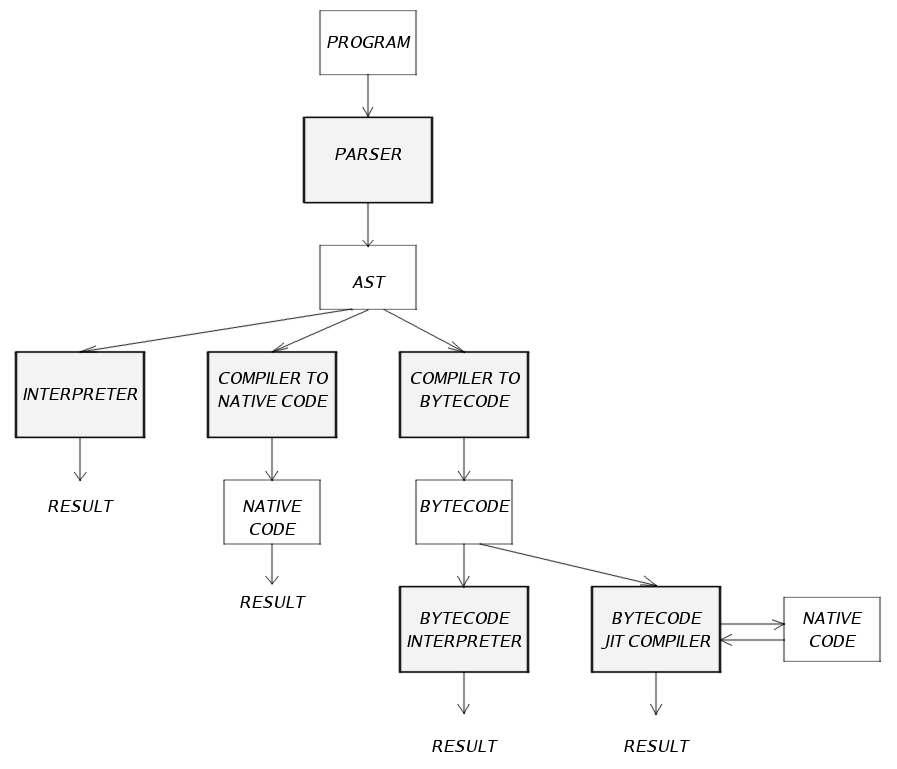
\includegraphics[width=4in]{pic/scheme.png}
\\
Все языковые процессоры будут использовать общий парсер.
Парсер будет генерировать AST.
Каждый языковой процессор будет рекурсивно обходить AST и делать что-то своё:
выполнять программу, генерировать машинные инструкции, генерировать байткод виртуальной машины.
Чего в нашем примере не будет --- так это оптимизаций (слишком простой язык).

\section{Грамматика}
Язык я выберу очень простой: арифметические операции над целыми числами
в десятичном представлении. Этот язык можно описать такой грамматикой $G=<V,W,P,S>$:

$$V=\{0,1,2,3,4,5,6,7,8,9,+,-,*,/,(,)\}$$
$$W=\{digit, number, factor, term, expr\}$$
$$P=\left\{
\begin{array}{l l}
digit \  & \rightarrow \ 0 \ | \ 1 \ | \ 2 \ | \ 3 \ | \ 4 \ | \ 5 \ | \ 6 \ | \ 7 \ | \ 8 \ | \ 9
\\
number \  & \rightarrow \ digit \ number \ | \ digit
\\
factor \  & \rightarrow \ number \ | \ ( expr )
\\
term \  & \rightarrow \ term * factor \ | \ term / factor \ | \ factor
\\
expr \  & \rightarrow \ expr + term \ | \ expr - term \ | \ term
\end{array}
\right. $$
$$S=expr$$
\\
Эта грамматика может показаться сложноватой.
Во-первых, вместо трёх правил для нетерминалов $factor$, $term$ и $expr$ можно обойтись
одним:
$$expr \  \rightarrow \ expr + expr \ | \ expr - expr \ | \ expr * expr \ | \ expr / expr \ | \ ( expr ) \ | \ number$$
\\
Это правило позволяет описывать те же самые языковые конструкции, что и три правила $factor$, $term$ и $expr$ вместе взятые.
Кроме того, оно проще и очевиднее. Зачем разбивать его на три? А вот зачем:
такое разделение позволяет прямо в грамматике закодировать \emph{приоритеты} арифметических операций.
У скобок самый большой приоритет (правило $factor$); затем идут мультипликативные операции с меньшим приоритетом (правило $term$);
затем аддитивные с ещё меньшим приоритетом (правило $expr$). Получается, что трёхуровневые правила
описывают тот же \emph{синтаксис}, что и одноуровневое, но при этом описывают часть \emph{семантики} языка
(приоритет арифметических операций).
\\ \\
Вторая странность нашей грамматики, это то, что правила для арифметических операций имеют вид
$a \rightarrow a \circ b$. Возьмём, например, правило для сложения:
$expr \rightarrow expr + term$. Почему не $expr \rightarrow term + expr$ ? Или самый очевидный
вариант: $expr \rightarrow expr + expr$ ? Все три варианта описывают синтаксически эквивалентные языковые конструкции.
Чем первый вариант лучше? Дело тут в другой семантической особенности
нашего языка: \emph{левоассоциативность} бинарных операторов вычитания и деления.
Выражение ``$1 - 2 - 3$'', к примеру, следует понимать как ``$(1 - 2) - 3$'', а не ``$1 - (2 - 3)$''.
Рассмотрим повнимательнее правило для вычитания: $expr \rightarrow expr - term$.
Слева от ``$-$'' стоит $expr$, т.е. любое выражение. А вот справа --- $term$,
т.е. выражение, допускающее только мультипликативные операции над числами и выражениями в скобках.
Получается, такое правило заставляет нас однозначно понимать ``$1 - 2 - 3$'' как ``$(1 - 2) - 3$''.
Если бы мы выбрали правило $expr \rightarrow term - expr$, мы бы получили \emph{правоассоциативный}
оператор вычитания (и такие операторы иногда нужны). А вот третье правило, $expr \rightarrow expr - expr$,
вообще \emph{неоднозначное}: оно позволяет понимать выражение ``$1 - 2 - 3$''
двумя способами. Неоднозначность в грамматиках --- источних бед. Её следует допускать только тогда, когда
сам по себе язык неоднозначен (как, например, русская фраза ``он умеет заставить себя слушать'').
Кстати, правила для сложения и умножения могут быть как левоассоциативными, так и правоассоциативными, лишь бы не неоднозначными.
\\ \\
Итак, у нас есть очень хорошая и правильная грамматика: она не только
описывает всевозможные арифметические выражения, но ещё и придаёт им глубоко арифметический
смысл. Правильная грамматика --- это полдела, потому что благодаря ей мы
чётко понимаем, с чем мы имеем дело.

\section{Парсер}
Раз уж мы собрались строить языковые процессоры для языка арифметических
выражений, то начинать нужно с парсера. Парсер должен структурировать входную
строку в соответствии с нашей грамматикой:
\\ \\
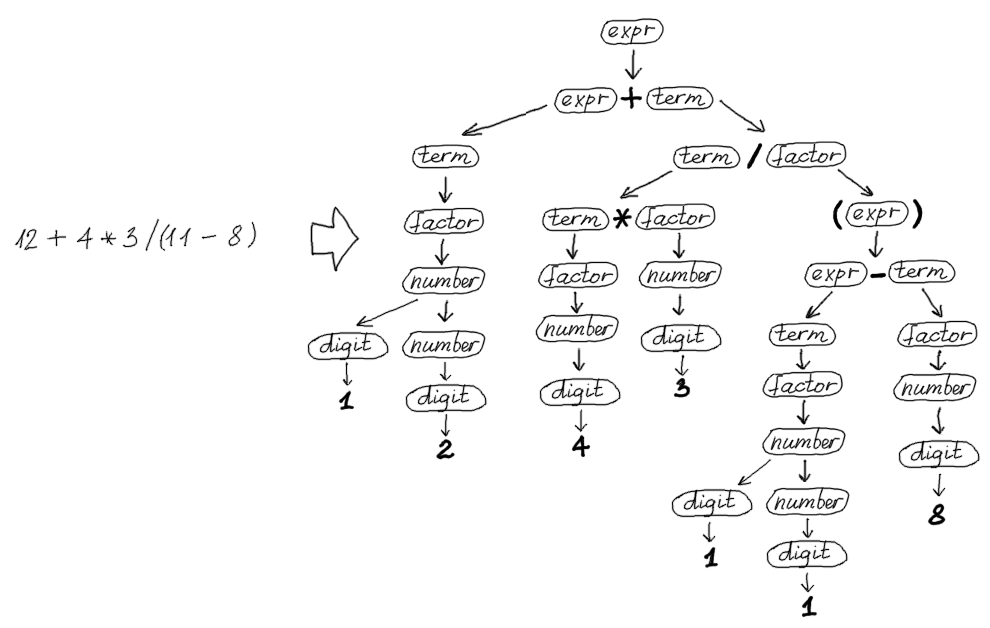
\includegraphics[height=3.5in]{pic/18.png}
\\ \\
Дерево на картинке --- это \emph{дерево разбора}.
Вообще, правильнее было бы говорить \emph{граф разбора}, потому что этот граф является деревом только для некоторых классов грамматик.
В нашем случае мы с полным правом можем говорить ``дерево''.
Возникает два вопроса:
\begin{enumerate}
\item Как заставить парсер догадаться, какая стуктура соответствует строке?
Явно придётся выковыривать символы, искать среди них плюсы, минусы и прочее.
Но как сделать это грамотно?
\item Допустим, парсеру каким-то чудом удалось распознать в строке
структуру. Что он должен делать с этим тайным знанием? Немедленно использовать
и тут же забыть? Или как-то сохранить для последующего использования?
\end{enumerate}
Разберёмся сначала с первым.
\\ \\
Один из самых простых подходов при написании парсера --- это так называемый \emph{метод
рекурсивного спуска} (recursive descent). Суть метода такая: для каждого нетерминала пишется
отдельная маленькая функция-парсер. Эта функция вызывает функции-парсеры для других нетерминалов (возможно, саму себя) ---
точно так же, как правила грамматики ссылаются друг на друга. В итоге
парсер структурно повторяет грамматику. Примерно так:

\lstinputlisting[language=Haskell]{example_recursive_descent/parser1_bad.hs}
Парсер написан на языке Haskell с использованием библиотеки Parsec.
Как видно из 1-й строки, мы взяли всего три библиотечных функции: \texttt{<|>}, \texttt{char} и \texttt{parse}.
Остальное --- встроенные хаскельные функции и операторы.
Оператор \texttt{<|>} работает как логическое \emph{или}: запускает левый парсер,
и если он отработал неудачно, запускает правый парсер.
Оператор \texttt{>\thinspace >} работает как логическое \emph{и}: запускает левый парсер,
и если он отработал удачно, запускает правый парсер.
Поскольку наш парсер пока не возвращает никакого результата (только проверяет синтаксическую корректность),
то все функции-парсеры должны возвращать значение типа \texttt{()} 
(аналог типа \texttt{void} в С/С++). Чтобы возвращать \texttt{()},
функция должна конце вызывать \texttt{return ()} или другую функцию, которая возвращает \texttt{()}.
\\ \\
Метод рекурсивного спуска --- это очень простой метод
построения парсеров, наиболее \emph{естественный} для человека: он позволяет писать парсер почти не задумываясь,
просто глядя на грамматику. На практике у этого метода есть две основные проблемы.
\\ \\
Первая проблема --- корректный перебор нескольких альтернатив. Если не сработал первый парсер, надо не просто
запустить второй, но ещё и перед этим аккуратно откатить назад все изменения, сделанные первым (backtrack).
В частности, если первый парсер продвинулся на несколько символов во входной строке,
то надо вернуться на прежнюю позицию. В библиотеке Parsec для этого есть функция \texttt{try}:
она запоминает состояние, к которому нужно откатиться.
С учётом функции \texttt{try} парсер выглядит так:
\lstinputlisting[language=Haskell]{example_recursive_descent/parser2_better.hs}
Обрати внимание, что \texttt{try} нужно вставлять перед всеми альтернативами,
кроме последней: если она не сработает, весь парсер не сработает. Кроме того, \texttt{try}
не надо вставлять, если альтернатива проверяет не больше одного символа.
\\ \\
Вторая проблема --- левая рекурсия в грамматике. Например, правило $expr \rightarrow expr - term$ леворекурсивное,
потому что крайний левый символ правой части --- это сам определяемый нетерминал.
Понятно, что если функция-парсер \texttt{expr} первым делом начнёт
вызывать саму себя (что она и делает), то программа в лучшем случае зациклится (а в худшем сожрёт память и упадёт).
Есть два пути решения этой проблемы:
    \begin{enumerate}
    \item Перестраивать грамматику при помощи формального алгоритма избавления от левой рекурсии.
    Этот подход гарантирует, что порождаемый грамматикой язык не изменится, и что левой рекурсии
    не будет. Из недостатков --- грамматика станет не такой красивой и удобной. Зато этот алгоритм
    универсальный.
    \item Вставлять костыли в парсер. В простых случаях удаётся ``на глаз'' переписать функцию-парсер так,
    чтобы она по смыслу делала то же самое, но не зацикливалась. В общем случае есть формальные
    алгоритмы, позволяющие грубой силой или хитростью ограничивать левую рекурсию, но эти
    алгоритмы довольно сложные и кривые.
    \end{enumerate}
Пойдём первым путём: применим к грамматике формальный алгоритм устранения левой рекурсии.
Наш случай простой: мы имеем дело с
\emph{непосредственной} левой рекурсией, т.е. правилом вида $A \rightarrow A \alpha$.
(Бывает ещё \emph{косвенная} левая рекурсия, образованная не одним, а несколькими правилами:
например $A \rightarrow B \alpha$, $B \rightarrow A \beta$.) Алгоритм избавления от непосредственной
левой рекурсии очень простой: каждое леворекурсивное правило $A \rightarrow A \alpha_1 | ... | A \alpha_n | \beta_1 | ... | \beta_m$
заменяется парой правил $A \rightarrow \beta_1 A_1 | ... | \beta_m A_1$,
$A_1 \rightarrow \alpha_1 A_1 | ... | \alpha_n A_1 | \epsilon$, где $A_1$ --- новый нетерминал.
В нашей грамматике леворекурсивных правила два: $term$ и $expr$. Изменённая грамматика
имеет вид:

$$V=\{0,1,2,3,4,5,6,7,8,9,+,-,*,/,(,)\}$$
$$W=\{digit, number, factor, term, term_1, expr, expr_1\}$$
$$P=\left\{
\begin{array}{l l}
digit \  & \rightarrow \ 0 \ | \ 1 \ | \ 2 \ | \ 3 \ | \ 4 \ | \ 5 \ | \ 6 \ | \ 7 \ | \ 8 \ | \ 9
\\
number \  & \rightarrow \ digit \ number \ | \ digit
\\
factor \  & \rightarrow \ number \ | \ ( expr )
\\
term \  & \rightarrow \ factor \ term_1
\\
term_1 \  & \rightarrow \ * factor \ term_1 \ | \ / factor \ term_1 \ | \ \epsilon
\\
expr \  & \rightarrow \ term \ expr_1
\\
expr_1 \  & \rightarrow \ + term \ expr_1 \ | \ - term \ expr_1 \ | \ \epsilon
\end{array}
\right. $$
$$S=expr$$
\\
Алгоритм гарантирует, что новая грамматика порождает в точности тот же язык,
что и старая (в том числе сохранилась семантика приоритетов и ассоциативности). Парсер для новой грамматики
отличается от старого парсера \emph{точно так же}, как новая грамматика отличается от старой:

\lstinputlisting[language=Haskell]{example_recursive_descent/parser3_best.hs}
Как хорошо! Все изменения сделаны автоматически, поэтому ошибки маловероятны.
Если б мы попытались переписать парсер руками, пришлось бы думать и хитрить, и
не было бы этой замечательной уверенности, что всё сделано правильно.
Мы сохранили главное: близость парсера к грамматике. До тех пор, пока парсер
соответствует грамматике, он остаётся \emph{понятным} и его \emph{легко менять},
изменяя  грамматику. Но как только парсер отдалится от грамматики,
он навсегда погрязнет в болоте сомнительных костылей и чудом работающих хаков.
\\ \\
На этом с синтаксическим разбором всё: у нас есть алгоритм написания парсера (метод рекурсивного спуска)
и грамматика, хорошо подходящая для этого алгоритма. Дальше по этой теме читай в книжке Grune, Jacobs: ``Parsing Technique. A Practical Guide'' --- там
приводится полная классификация алгоритмов синтаксического разбора со всеми их слабыми и сильными местами.
\\ \\
Теперь вернёмся ко второму вопросу: в каком виде парсер должен возвращать результат?
Очевидно, это зависит от того, что мы понимаем под результатом. Если нужно просто
проверить синтаксическую корректность выражения, можно ничего не возвращать.
Если мы хотим \emph{вычислить} значение выражения, то придётся следить
за частично вычисленным значением. Если мы хотим \emph{скомпилировать} выражение
в программу на другом языке (или в байткод виртуальной машины), нужно таскать за собой
буфер и дописывать туда новые инструкции. В общем, в каждом конкретном случае
нужно что-то своё.
\\ \\
Можно написать по отдельному парсеру на каждый случай. Но это немного обидно:
самая сложная часть парсера (синтаксический разбор) будет везде повторяться.
Чтобы этого избежать, мы введём промежуточное представление: AST. Парсер будет
строить AST, а потом уже с этим AST можно делать всё, что угодно:
вычислять значение выражения, генерировать инструкции, проводить сложные оптимизации и т.д.
(Важное замечание: поскольку наш язык очень простой, он допускает \emph{прямую} интерпретацию
и компиляцию: прямо по ходу синтаксического разбора, из парсера, можно сделать
всё, что надо. Промежуточное представление для нас --- просто удобный способ не дублировать код.
В более сложных случаях без него не обойтись.)
\\ \\
Какой должна быть структура AST для нашего языка?
Самый простой вариант --- дерево разбора. В начале главы мы уже смотрели на дерево разбора
для выражения $12 + 4 * 3 / (11 - 8)$. Вот как оно выглядит
после избавления от левой рекурсии в грамматике:
\\ \\
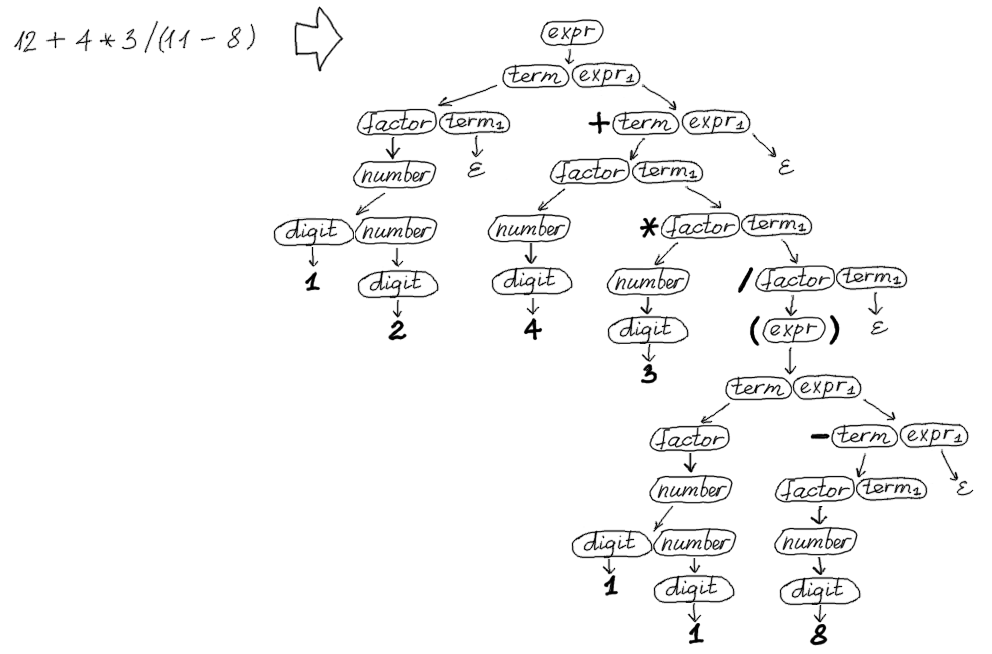
\includegraphics[height=3.5in]{pic/19.png}
\\ \\
Дерево разбора представляет структуру арифметического выражения в точном соответствии с грамматикой.
Это дерево хорошее и правильное, но какое-то оно \emph{слишком детальное}.
Например, чтобы добраться до числа $12$, надо обойти вершины $expr$, $term \ expr_1$, $factor \ term_1$ и $number$,
а потом ещё по кускам собирать само число из цифр, сидящих в вершинах $digit$.
Зачем нам хранить в AST информацию, что число $12$ получилось таким хитрым путём?
Ненужная детализация --- это источник бед. Во-первых, она дурит голову (например,
я размазываю простенький пример на десять страниц, и ты не улавливаешь сути). Во-вторых,
все эти детали надо где-то хранить (для больших выражений потребуется уйма памяти).
В-третьих, обходя огромное дерево, больше шансов где-то сделать ошибку.
\\ \\
Человек представляет себе выражение $12 + 4 * 3 / (11 - 8)$ вот так:
\\ \\
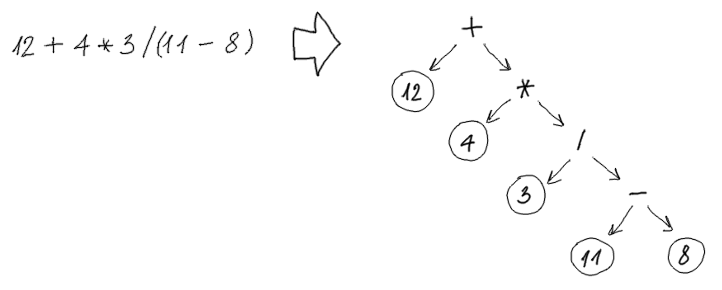
\includegraphics[height=2in]{pic/20.png}
\\ \\
Это дерево отражает структуру выражения ничуть не хуже,
чем дерево разбора, но при этом оно намного проще и компактнее. Почему мы не можем
сделать дерево разбора таким же простым? Дерево разбора зависит только от грамматики.
Чтобы дерево разбора было красивым, нужна другая, красивая грамматика. К несчастью,
красивые грамматики обычно напичканы неоднозначностями, и парсер для них написать
очень трудно или вообще невозможно (кроме того, такие парсеры работают очень медленно).
Наша грамматика некрасивая, потому что она приспособлена для компьютера, а не для человека.
Но никто не мешает нам сделать AST не таким, как дерево разбора.
\\ \\
Итак, в нашем AST будут узлы пяти типов: ``число'', ``плюс'', ``минус'', ``умножить'', ``поделить''.
Узел типа ``число'' всегда будет листом, т.е. у него не будет детей. У остальных типов
узлов будет ровно по два ребёнка: левый и правый операнды. Узлы-операнды могут быть числом
(если тип узла - ``число'') или корнем поддерева (если тип узла --- ``плюс'', ``минус'', ``умножить'' или ``поделить'').
На хаскеле такой тип данных выражается проще некуда:
\begin{verbatim}
data AST
    = Number Int
    | Add AST AST
    | Sub AST AST
    | Mul AST AST
    | Div AST AST
\end{verbatim}
Здесь \texttt{AST} --- тип данных, который мы определяем;
\texttt{Int} --- встроенный хаскельный тип; \texttt{Number},
\texttt{Add}, \texttt{Sub}, \texttt{Mul} и \texttt{Div} ---
функции-конструкторы нашего типа \texttt{AST}. Конструктор может принимать аргументы, как и любая функция:
в нашем случае конструктор \texttt{Number} --- это функция, принимающая один аргумент типа \texttt{Int},
а конструкторы \texttt{Add}, \texttt{Sub}, \texttt{Mul} и \texttt{Div} ---
функции, принимающие по два аргумента типа \texttt{AST}. Определения для этих функций писать не надо:
они настолько очевидные, что компилятор сгенерирует их сам.
Теперь сделаем так, чтоб наш парсер сохранял результаты разбора в структуру AST:
\lstinputlisting[language=Haskell]{example_recursive_descent/parser4_ast.hs}
Раньше нас не интересовал результат работы парсера: всё наши
функции-парсеры возвращали значение типа \texttt{()}. Теперь каждая функция-парсер возвращает результат
своей работы: функции \texttt{digit} и \texttt{number} возвращают результат типа \texttt{Int},
а остальные --- результат типа \texttt{AST}. Функции \texttt{expr1} и \texttt{term1}
теперь принимают параметр типа \texttt{AST} --- левый операнд. Затем они пытаются распарсить правый операнд,
и если это удаётся, то из двух операндов строится новый \texttt{AST}, а если нет --- возвращается левый
операнд. Функция \texttt{number} теперь принимает один аргумент типа \texttt{Int} --- частично вычисленное число.
\\ \\
В тех местах, где возвращаемое из парсера значение важно, вместо оператора \texttt{>\thinspace >}
используется очень похожий оператор \texttt{>\thinspace >=}. Отличие этих двух операторов в том, что \texttt{>\thinspace >}
игнорирует значение, возвращаемое первым парсером, а \texttt{>\thinspace >=} передаёт это значение
второму парсеру в качестве аргумента. Иногда надо не просто передать значение второму парсеру,
а как-то более хитро его использовать.
Чтобы как-то назвать, \emph{обозначить} это возвращаемое значение, используется синтаксис \emph{лямбда-функции}:
\texttt{\textbackslash <arguments> -> <calculations with arguments>}.
\\ \\
\texttt{deriving (Show)} (строка 9) говорит компилятору, что надо сгенерировать функции для вывода
значений типа \texttt{AST} на экран. Без этого мы не смогли бы распечатать полученный \texttt{AST}
(строка 44).
\\ \\
Если что-то непонятно в этом исходнике --- не переживай. Здесь уже слишком много хаскельного сиснтакса,
чтобы всё сразу было понятно. Я привожу примеры на хаскеле по двум причинам: во-первых, потому что
на хаскеле они короткие и способствуют пониманию алгоритма; во-вторых, чтоб заинтересовать тебя.
\\ \\
Теперь напишем тот же самый парсер на С++. Вот как выглядит структура \texttt{AST} (файл ast.h):
\lstinputlisting[language=C++]{example_lang_proc/ast.h}
В файле ast.cpp находится реализация конструкторов и деструкторов \texttt{AST}:
\lstinputlisting[language=C++]{example_lang_proc/ast.cpp}
Теперь перейдём к самому парсеру. По сути он мало отличается от хаскельного
парсера, хотя и не такой элегантный. На C++ нам надо вручную следить
за продвижением указателя во входной строке, поэтому мы передаём его первым аргументом
во все функции (в хаскеле это неявно делала библиотека Parsec).
Обрати внимание, что указатель везде передаётся \emph{по ссылке}, поэтому все изменения, которые делает с ним \emph{вызываемая}
функция, становятся видны \emph{вызывающей} функции. Вот прототипы
функций-парсеров (parser.h):
\lstinputlisting[language=C++]{example_lang_proc/parser.h}
А вот их реализации (parser.cpp):
\lstinputlisting[language=C++]{example_lang_proc/parser.cpp}
Вот и всё! Парсер готов. Он, конечно, далеко не идеален (в частности, плохо обрабатывает ошибки).
Но больше мы его менять не будем.

\section{Интерпретатор}
Интерпретатор выглядит до смешного просто. Вот его прототип (файл interpreter.h):
\lstinputlisting[language=C++]{example_lang_proc/interpreter.h}
А вот реализация (файл interpreter.cpp):
\lstinputlisting[language=C++]{example_lang_proc/interpreter.cpp}
Функция \texttt{interpret} определяет тип узла: если это \texttt{NUMBER},
то нужно просто вернуть соответствующее число; иначе нужно рекурсивно вычислить
значение левого и правого операндов и вернуть результат операции над ними.

\section{Компилятор}
Компилятор структурно не сложнее интерпретатора: он точно так же рекурсивно обходит
\texttt{AST}, только вместо немедленного вычисления генерирует машинные инструкции.
Первым делом надо решить важный вопрос: для какой архитектуры?
\\ \\
Архитектура компьютера --- понятие широкое. Нас интересует \emph{архитектура как набор команд процессора} 
(Instruction Set Architecture, ISA). Можно сделать два совершенно
разных процессора, которые будут понимать один и тот же набор команд. Компилятор не увидит
разницы меду ними: ему всё равно, как процессор устроен физически.
Единственное, что компилятору надо знать --- это какие команды понимает процессор
и насколько эффективно он выполняет конкретную команду. Поэтому, говоря об
архитектуре, я имею в виду набор команд процессора.
\\ \\
Какую архитектуру нам выбрать? В принципе, \emph{любую}. Можно, к примеру, выбрать
исторически первый компьютер и компилировать в машинный код для него. 
Только вот запустить такую программу будет негде, поэтому лучше выбрать 
архитектуру твоего компьютера. Кстати, что это за архитектура?
\\ \\
Это можно узнать несколькими способами. Например, поискать в интернетах спецификацию
этой модели (Lenovo ThinkPad X220i). Привожу её тут полностью (вдруг что полезное узнаешь про свой комп),
но нас интересует только секция ``Processor / Chipset'':

\begin{scriptsize}
\begin{verbatim}
Lenovo ThinkPad X220i

    Processor / Chipset
        CPU                                 Intel Core i3 (2nd Gen) 2310M / 2.1 GHz
        Number of Cores                     Dual-Core
        Cache                               L3 - 3 MB
        64-bit Computing                    Yes
        Chipset                             Mobile Intel QM67 Express
        Features                            Intel Turbo Boost Technology 2.0
\end{verbatim}
\end{scriptsize}

\begin{tiny}
\begin{verbatim}
    Memory
        Max RAM Supported                   8 GB
        Technology                          DDR3 SDRAM
        Speed                               1333 MHz / PC3-10600
        Form Factor                         SO DIMM 204-pin
        Slots Qty                           2
        Empty Slots                         1

    Storage
        Interface                           Serial ATA-300

    Display
        LCD Backlight Technology            LED backlight
        Widescreen                          Yes
        Image Aspect Ratio                  16:9
        Features                            anti-glare

    Audio & Video
        Graphics Processor                  Intel HD Graphics 3000
        Memory Allocation Technology        Dynamic Video Memory Technology
        Camera                              Yes
        Resolution                          0.92 Megapixel
        Capture Resolutions                 1280 x 720
        Sound                               Stereo speakers , stereo microphone
        Codec                               CX20672
        Compliant Standards                 High Definition Audio

    Input
        Type                                touch-screen
        Features                            spill-resistant

    Communications
        Wireless                            Bluetooth 3.0
        Wireless Controller                 Intel Centrino Wireless-N 1000
        Network Interface                   Gigabit Ethernet

    Wireless Broadband (WWAN)
        Generation                          3G upgradable

    Battery
        Installed Qty                       1
        Max Supported Qty                   2
        Run Time                            8.8 sec

    AC Adapter
        Input                               AC 120/230 V ( 50/60 Hz )
        Output                              65 Watt

    Connections & Expansion
        Slots                               1 x ExpressCard/54 ( 1 free )
        Interfaces                          2 x USB 2.0
                                            PoweredUSB
                                            VGA
                                            DisplayPort
                                            LAN
                                            Headphone/microphone combo jack
                                            Dock
        Memory Card Reader                  3 in 1 ( SD Card, SDHC Card, SDXC Card )

    Software
        Software Included                   ThinkVantage Toolbox
        Microsoft Office Preloaded          Includes a pre-loaded image of select Microsoft Office
                                            suites. Purchase an Office 2010 Product Key Card or
                                            disc to activate preloaded software on this PC.

    Miscellaneous
        Security                            Trusted Platform Module (TPM 1.2) Security Chip,
                                            fingerprint reader
        Features                            Intel Active Management Technology (iAMT)
        Compliant Standards                 RoHS
        Manufacturer Selling Program        TopSeller

    Dimensions & Weight
        Width                               12 in
        Depth                               9 in
        Height                              1.2 in
        Weight                              3.7 lbs

    Environmental Standards
        ENERGY STAR Qualified               Yes

    Sustainability
        ENERGY STAR Qualified               Yes
        Greenpeace policy rating (Nov 2011) 3.8

    General
        Manufacturer                        Lenovo
\end{verbatim}
\end{tiny}
Видно, что процессор у тебя --- Intel Core i3, двухъядерный и 64-разрядный. Описание
архитектуры этого процессора найти несложно.
\\ \\
Другой, линуксоспецифичный, способ --- выполнить одну из
команд \texttt{arch}, \texttt{uname -m}, \texttt{lscpu}, \texttt{cat /proc/cpuinfo} или ещё какую-нибудь.
Команды \texttt{arch} и \texttt{uname -m} просто бесхитростно пишут название архитектуры (эти команды идентичны).
Команда \texttt{lscpu} выводит больше информации о процессоре,
а команда \texttt{cat /proc/cpuinfo} выводит информацию про каждое ядро в отдельности.
\\ \\
Но что, если ты не знаешь модель (нашла компьютер в канаве), и операционная система на нём
очень глупая? Можно попробовать расковырять исполняемый файл какой-нибудь программы, которая запускается
на этом компьютере. Попытаться понять, что там за инструкции (не самый лёгкий способ).
Можно пытаться запустить программы для разных архитектур (пока компьютер не взорвётся).
Если компьютер после этих экспериментов больше не включается, можно расковырять его внутренности.
В общем, есть способы.
\\ \\
У меня есть основания предполагать, что архитектура твоего компьютера --- x86.
Как и моего, и вообще, большинства ноутбуков и десктопов, которые ты видишь.
Про эту архитектуру написано много, и я только вкратце упомяну только самое основное.
\\ \\
Программа --- это последовательность команд процессору.
Команды в основном работают с какими-то данными:
они могут принимать на вход \emph{операнды} и возвращать \emph{результат}.
Все эти данные надо где-то хранить.
С точки зрения программы есть три вида памяти:
\begin{enumerate}
\item \textbf{Регистры}
\\
Это маленький кусок сверхбыстрой памяти, зашитой внутри процессора.
Регистры нужны, чтобы не тратить время на доступ к оперативной памяти: загрузка/выгрузка данных выполняется значительно дольше, чем сама команда.
Регистры активно используются для хранения операндов и результатов команд.
Данные в них не задерживаются: они храняться там временно, чтобы вскоре быть использованными и затёртыми новыми данными.
Поскольку регистров мало, у каждого из них есть своё имя, и в командах регистры адресуются всего несколькими битами.
\item \textbf{Оперативная память}
\\
Оперативная память --- это большой кусок медленной памяти, внешней по отношению к процессору.
В оперативной памяти хранится сама программа и все данные, с которыми она работает.
Когда очередной кусок данных нужен для вычислений на процессоре, этот кусок загружается из оперативной памяти в регистры.
Окончательные результаты вычислений выгружаются назад в оперативную память.
Промежуточные результаты, если они не помещаются в регистры, тоже выгружаются в оперативную память.
Оперативная память --- это память с \emph{произвольным доступом} (Random Access Memory, RAM).
Это значит, что одновременно доступны все байты в этой памяти.
Адресом байта служит его порядковый номер.
Поскольку команда может обратиться к любому байту, адрес должен быть целиком зашит в команду.
\item \textbf{Стек}
\\
Стек --- это кусок оперативной памяти со специальными правилами доступа.
Как и оперативная память, стек медленный. Размер стека может быть разным: программа может ограничить себе стек или вообще отказаться от него.
Обычно максимальный размер стека ограничен операционной системой.
Доступ к стеку осуществляется по правилу LIFO (Last In, First Out): одновременно доступно только одно значение (вершина стека).
Адрес вершины стека хранится в специальном регистре, и команды, работающие со стеком, используют этот регистр.
Стек нужен для удобства программистов.
\end{enumerate}
\bigskip
\begin{minipage}{0.6\textwidth}
Физически иерархия памяти устроена более сложно:
между регистровой и оперативной памятью есть ещё несколько уровней \textbf{кэш-памяти}.
В кэш загружаются те данные, которые не попали в регистры, но предположительно скоро понадобятся.
Когда нужны какие-то данные из оперативной памяти, первым делом они ищутся в кэше:
если они там есть (cache hit) --- отлично, если нет (cache miss) --- плохо, придётся тратить время на доступ к памяти.
Программист не управляет кэшами напрямую, как регистрами и оперативной памятью (и может вообще не знать об их существовании).
Есть команды, позволяющие влиять на кэширование данных, но в общем процессор оставляет за собой свободу действий.
\\ \\
Картинка примерно соответствуют семейству процессоров Intel Core
(подробнее о кэшах в мануале ``Intel 64 and IA-32 Architectures Optimization Reference Manual'').
\end{minipage}
\begin{minipage}{0.4\textwidth}
\centering
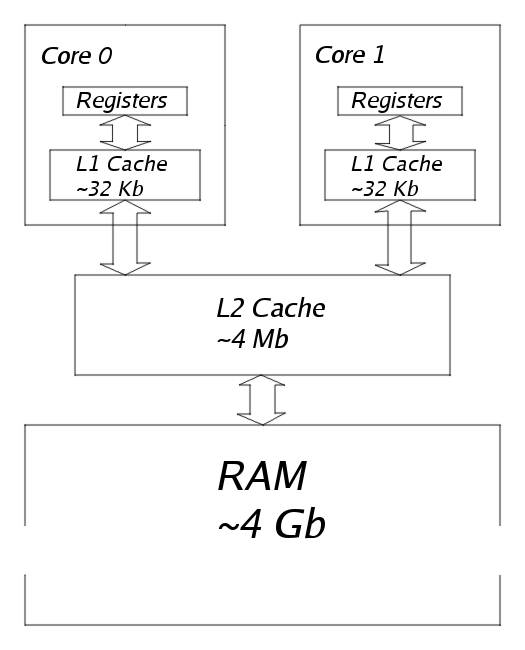
\includegraphics[width=\textwidth]{pic/caches.png}
\end{minipage}
\bigskip
\\
Регистры не безразмерные: каждый регистр рассчитан на хранение определённого числа битов.
В $N$-битном регистре можно сохранить $2^N$ различных значений.
Это могут быть целые беззнаковые числа в диапазоне $[0, 2^N - 1]$,
или целые числа со знаком в диапазоне $[-2^{N-1}, 2^{N-1} - 1]$,
или адреса байтов в памяти объёмом $2^N$ байт,
или что угодно ещё.
Важно, как понимает эти биты команда, которая работает с регистром.
Размер регистров ограничивает диапазон данных, с которыми работает процессор: данные, которые не влазят в этот диапазон, приходится обрабатывать по кускам.
Число битов в единице данных, с которой работает процессор, определяет его \textbf{разрядность}.
\\ \\
Как и с памятью, физическое устройство регистров может сильно отличаться от логического:
один логический регистр может состоять из нескольких физических или занимать только часть физического.
Некоторые логические регистры вообще не являются регистрами в физическом смысле (скорее набором управляющих сигналов).
В этом смысле разрядность процессора --- понятие сложное и неоднозначное.
Команды работают с логическими регистрами, поэтому нам, как программистам, важно логическое устройство процессора.
\\ \\
Архитектура x86 начиналась с 16-разрядного процессора 8086, сделанного компанией Intel в 1978 году.
Постепенно в неё добавлялись новые возможности: увеличивался размер регистров, появлялись новые регистры, расширялся набор команд.
При этом сохранялось важное свойство: более новые архитектуры x86 были \emph{обратно совместимы} с предыдущими (то есть понимали программы для предыдущих).
Обратная совместимость --- очень полезное свойство: не нужно переписывать старые программы, чтобы запустить их на новом процессоре.
С другой стороны, из-за обратной совместимости приходится таскать за собой много ненужного устаревшего хлама,
что значительно усложняет и замедляет процессор.
У твоего ноутбука 64-разрядная архитектура x86, сокращённо x86-64.
\\ \\
Примерно так выглядят регистры процессора x86-64:
\\
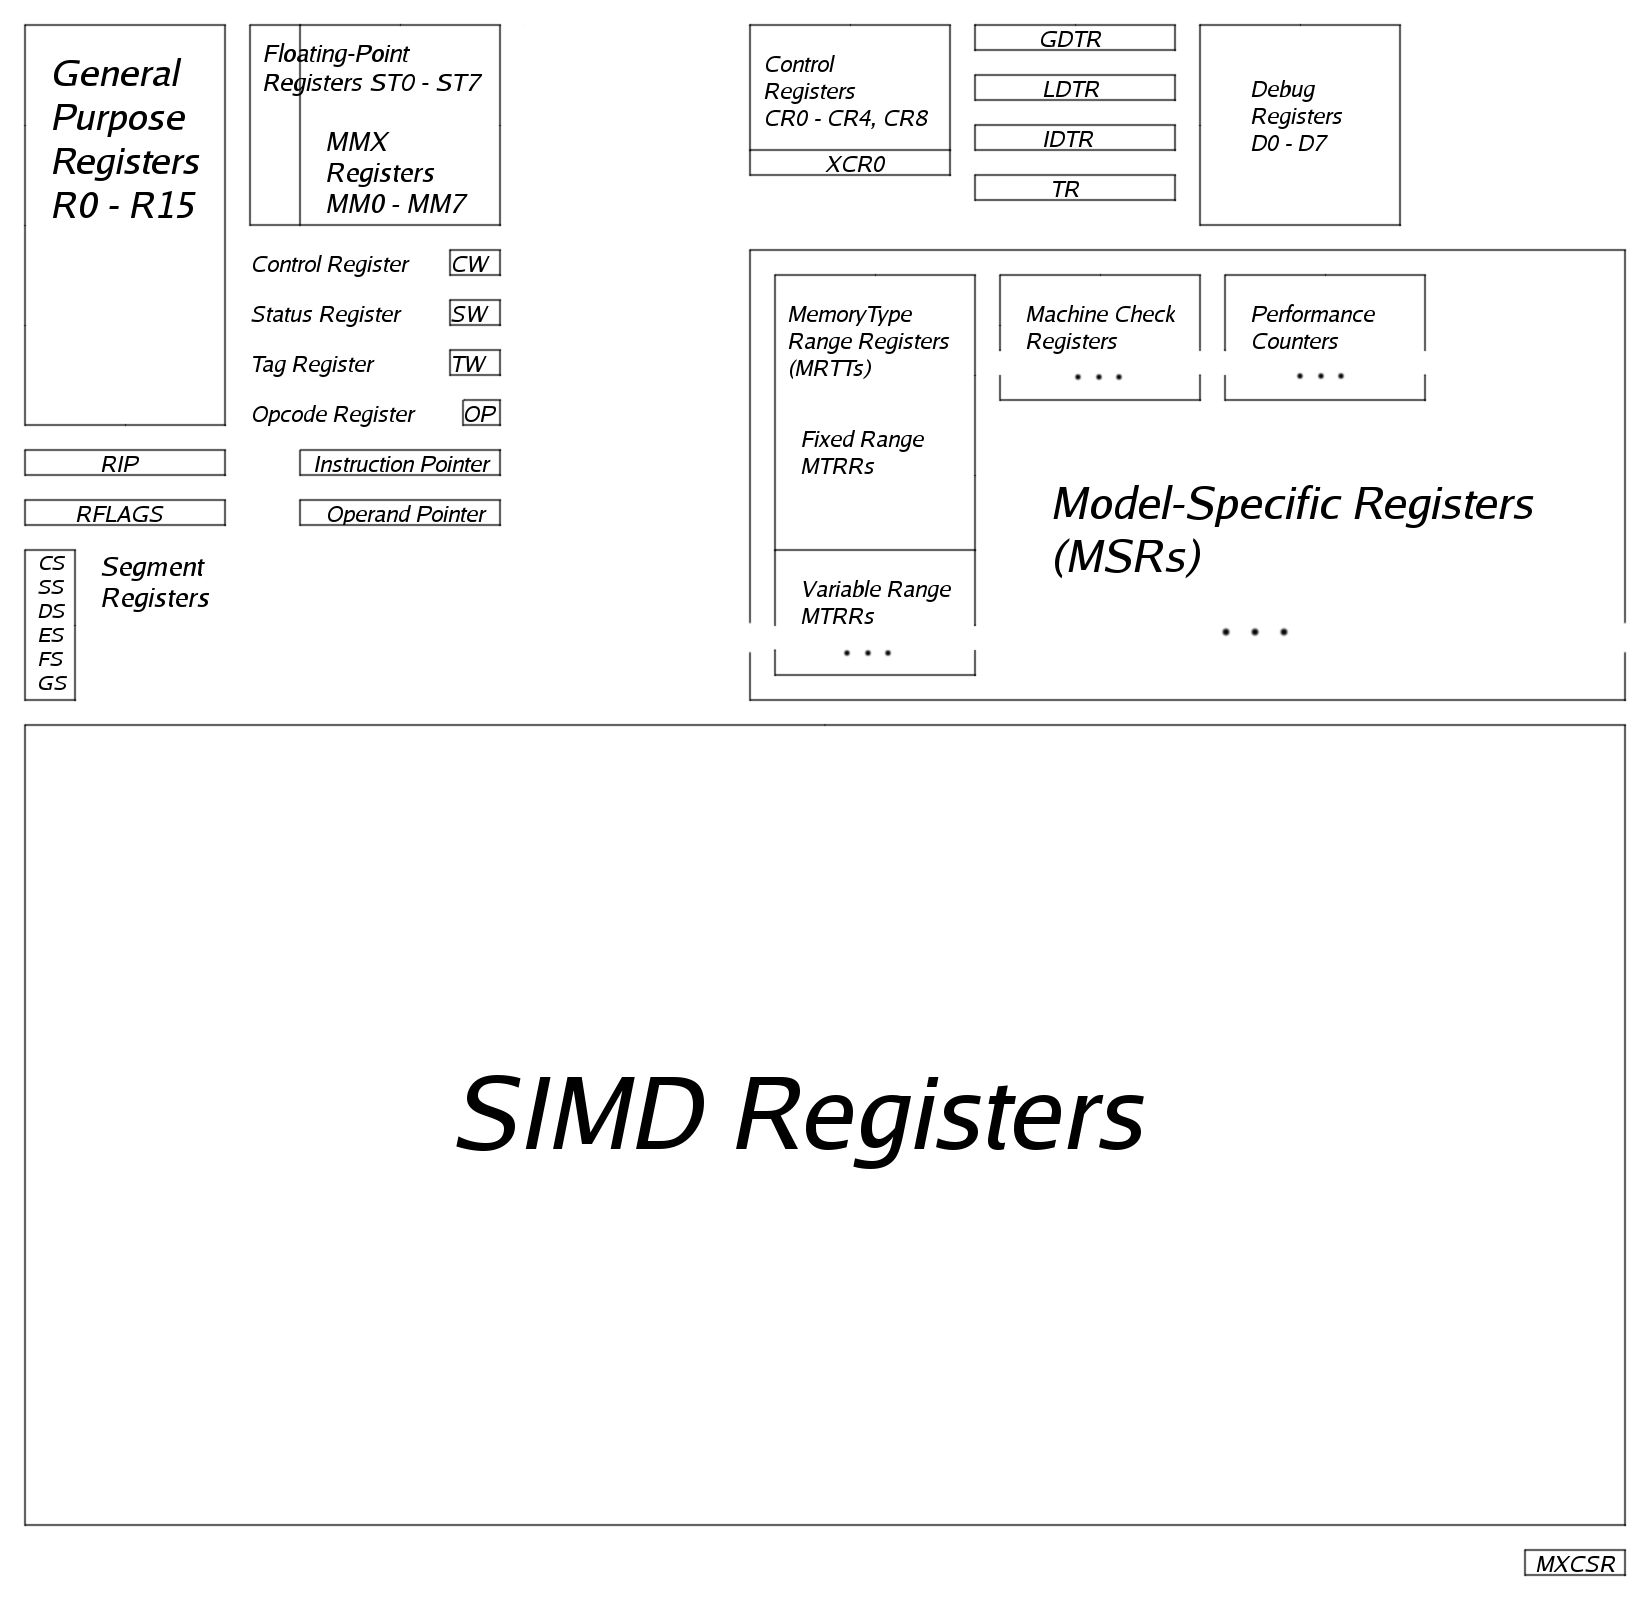
\includegraphics[width=6.5in]{pic/registers.png}
\\
На этой картинке сохранён относительный размер регистров (кроме MSR-ов, размер и число которых зависит от конкретной модели процессора).
Итого есть следующие важные группы регистров:
\begin{itemize}
\item Регистры общего назначения (General Purpose Registers, GPRs).
Это основные регистры, с которыми работает программист:
в них хранятся операнды, результаты команд и вообще всё, что угодно.
Их шестнадцать штук, каждый по 64 бита:
\\
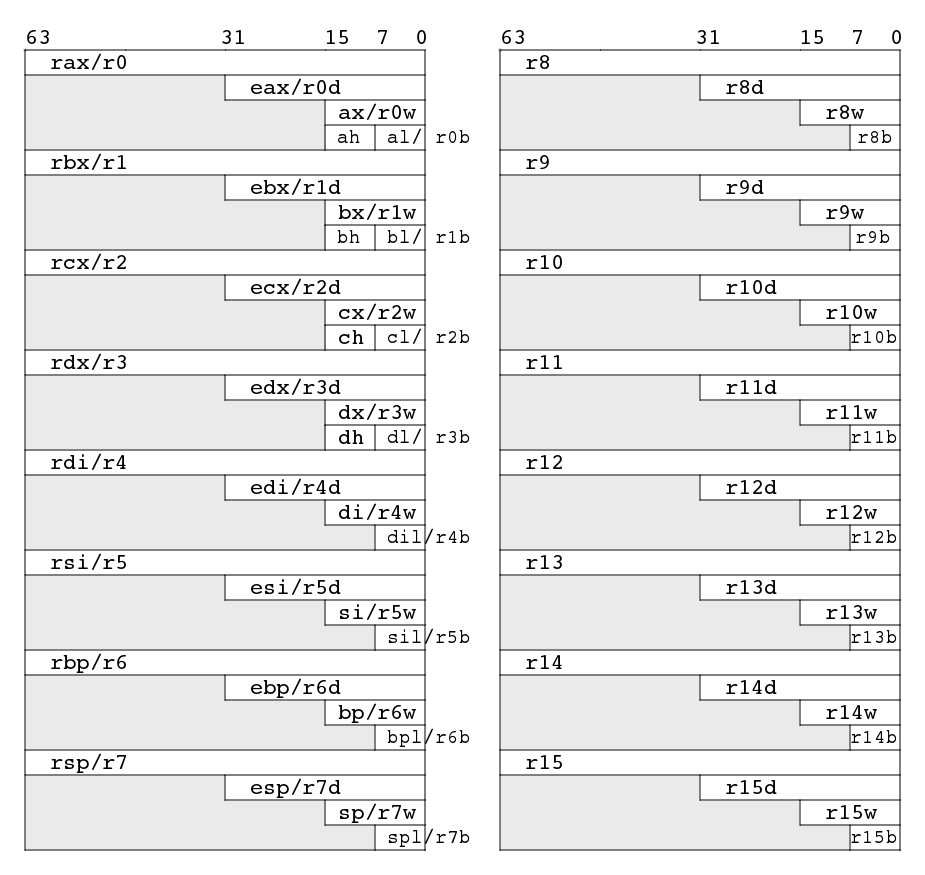
\includegraphics[height=5in]{pic/registers_general_purpose.png}
\\
$i$-й регистр называется $R_i$,
его младшая $32$-битная половина --- $R_iD$ (Double Word).
младшая $16$-битная четверть --- $R_iW$ (Word),
младшая $8$-битная восьмушка --- $R_iB$ (Byte).
Исторически сложилось так, что у первых восьми регистров есть личные имена: RAX, RBX, RCX, RDX, RDI, RSI, RBP и RSP
($32$-битные половины называются EAX, EBX, ECX, EDX, EDI, ESI, EBP и ESP, $16$-битные четверти --- AX, BX, CX, DX, DI, SI, BP и SP,
а $8$-битные восьмушки --- AL, BL, CL, DL, DIL, SIL, BPL и SPL).
Кроме того, старшие байты регистров AX, BX, CX и DX тоже имеют личные имены: AH, BH, CH и DH.
Имена отражают специфику использования каждого из регистров: 'A' --- accumulator, 'B' --- base, 'C' --- counter, 'D' --- data,
'DI' --- destination index, 'SI' --- source index, 'BP' --- base pointer, 'SP' --- stack pointer.
Это не значит, что эти регистры обязательно использовать таким образом, просто некоторые команды придают им специальный смысл.
\item Регистр, хранящий адрес следующей команды (Instruction Pointer, RIP).
Это 64-битный регистр. Хранящийся в нём 64-битный адрес --- это номер байта в оперативной памяти,
с которого начинается следующая инструкция. Процессор исполняет инструкцию и продвигает указатель в регистре RIP.
Программист не может изменять значение регистра RIP напрямую: он должен вызвать специальную инструкцию передачи управления
(\texttt{JMP}, \texttt{Jcc}, \texttt{CALL}, \texttt{RET} и \texttt{IRET}).
Исполняя эту инструкцию, процессор сам передвинет указатель куда надо.
\item Регистр флагов (RFLAGS) --- специальный регистр, содержащий набор флагов. Каждый флаг занимает один-два бита и имеет какой-то специальный смысл.
Старшая половина битов зарезервирована (всегда нулевая). Младшая половина (EFLAGS) выглядит так:
\\
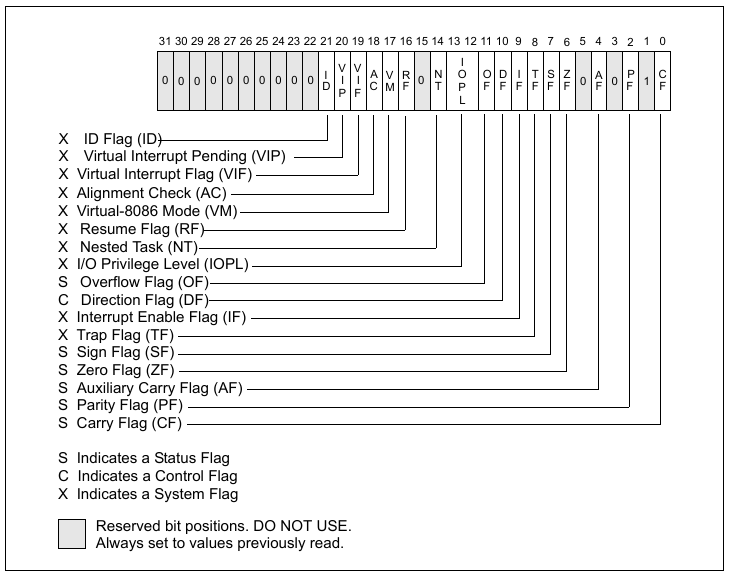
\includegraphics[height=4in]{pic/eflags.png}
\\
\item Сегментные регистры (CS, DS, SS, ES, FS, GS) --- регистры, содержащие адреса \emph{сегментов} памяти.
Физически оперативная память --- это просто массив байтов, и адрес в памяти --- это номер байта.
Логически может быть удобно представлять память как-то по-другому (или вообще использовать разные логические представления в зависимости от случая).
Одно из таких логических представлений --- \emph{сегментная модель памяти}.
В этой модели адресное пространство процесса состоит из кусков --- сегментов.
Разные сегменты соответствуют разным областям физической памяти (которые могут перекрываться и совпадать).
Логический адрес, с которым работает программа, состоит из двух частей: \emph{селектора} и \emph{смещения}.
Селектор отвечает за сегмент, к которому относится адрес, а смещение --- за конкретный байт внутри сегмента.
Логический адрес преобразуется в физический по хитрым правилам.
\\ \\
Сегментная модель позволяет много вариаций в зависимости от числа и взаимного расположения сегментов.
Самая простая модель --- плоская (flat memory model): адресное пространство процесса расположено в одном сегменте.
Плоская модель позволяет забыть о сегментах и работать так, как будто их вообще нет.
Это вырожденный случай сегментирования, но сейчас в основном используется именно плоская модель.
Сегментирование было очень кстати в 16-разрядных процессорах, поскольку в помощью 16-битного адреса можно адресовать всего лишь $2^{16}$ байта
(то есть объём памяти, доступной программе --- всего 64 Кб).
Использование разных сегментов позволило расширить объём доступной памяти.
С переходом на 64-разрядную архитектуру необходимость в разных сегментах отпала: 64 бита позволяют адресовать $2^{64}$ байта,
и пока что используется только часть этих битов.
\\ \\
У процессора есть разные режимы, и в этих режимах используется разное логическое представление памяти.
Основой режим --- защищённый (protected mode) --- требует использования сегментной модели памяти.
Другое дело, что обычно все сегменты слиты в один, поэтому сегментирование незаметно.
Подробнее о режимах процессора и моделях памяти читай в мануале ``Intel 64 and IA-32 Architectures Software Developer's Manual'', том 3, глава 2.
\item Регистры для работы с числами с плавающей запятой (Floating Point Registers).
Это восемь 80-битных регистров, организованных в виде стека (ST0 - ST7).
К ним добавляются контрольные регистры: 16-битные CW (Control Word), SW (Status Word) и TW (Tag Word),
11-битный FP\_OPC (Opcode) и 64-битные FP\_IP (Instruction Pointer) и FP\_DP (Data Pointer).
Всё вместе устройство называется \emph{сопроцессором FPU} (Floating Point Unit), или расширением x87.
Подробнее о работе с FPU читай в мануале ``Intel 64 and IA-32 Architectures Software Developer's Manual'', том 1, глава 8.
\item Регистры для работы с векторными инструкциями (Scalar Instruction Multiple Data, SIMD).
Это регистры для проведения векторных операций: например, для одновременного сложения не одной, а четырёх пар чисел.
К ним относятся регистры MMX, физически совмещённые с регистрами FPU; регистры SSE, AVX и т.д.,
а также контрольный регистр MXCSR (Control/Status Register).
Подробнее о векторных инструкциях и расширениях для работы с ними читай в мануале ``Intel 64 and IA-32 Architectures Software Developer's Manual'', том 1, главы 9 - 14.
\item Системные регистры.
Это регистры, с которыми возятся в основном разработчики операционной системы.
Большинство из этих регистров с горем пополам описаны в мануале ``Intel 64 and IA-32 Architectures Software Developer's Manual'', том 3
(так что тебе придётся прочитать его, когда надумаешь писать операционную систему для x86).
Вот основные группы системных регистров:
    \begin{itemize}
    \item Контрольные регистры (Control Registers) CR0 - CR4, CR8, XCR0.
    Они определяют режим работы процессора и характеристики текущей исполняемой задачи.
    \item Регистры управления памятью (Descriptor Table Registers) GDTR, IDTR, LDTR, TR.
    Регистр IDTR хранит указатель на таблицу дескрипторов обработчиков прерываний IDT (Interrupt Descriptor Table).
    Регистр TR хранит информацию о текущей выполняемой задаче.
    Регистры GDTR и LDTR нужны при использовании сегментной модели памяти:
    они хранят указатели на таблицы сегментных дескрипторов GDT (Global Descriptor Table) и LDT (Local Descriptor Table).
    Эти таблицы участвуют в процессе преобразования логического адреса в физический:
    \\
    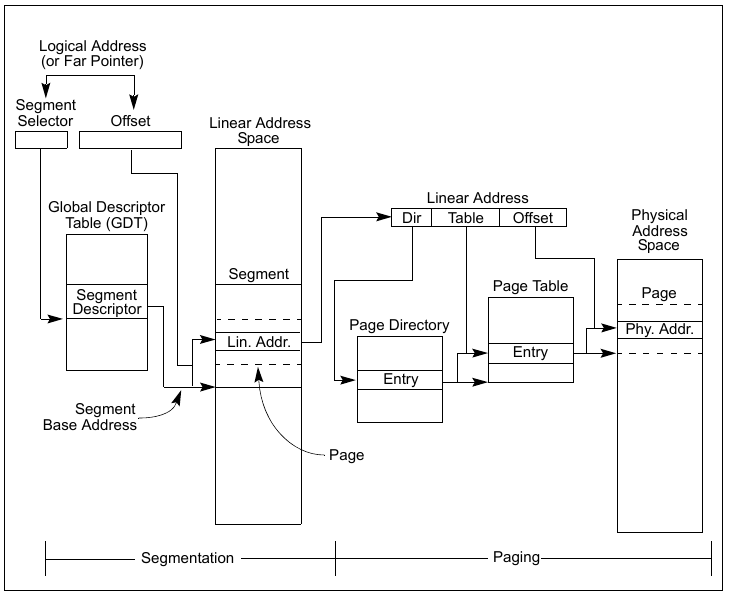
\includegraphics[height=3.5in]{pic/memory_management.png}
    \\
        \begin{enumerate}
        \item Логический адрес преобразуется в \emph{линейный} адрес.
        Процессор использует первую часть логического адреса --- селектор --- для чтения сегментного дескриптора из таблицы.
        Сегментный дескриптор содержит адрес начала сегмента в памяти (\emph{базовый} адрес) и атрибуты сегмента (размер, права доступа и т.д.).
        Процессор проверяет, попадает ли смещение (вторая половина логического адреса) внутрь сегмента и не нарушены ли права доступа к сегменту.
        Сумма базового адреса и смещения даёт линейный адрес.
        \item Линейный адрес преобразуется в физический адрес.
        Этот этап зависит от того, используется ли \emph{страничный механизм} управления памятью (paging).
        Страничный механизм --- это ещё одно логическое представление поверх сегментной модели памяти.
        Оно нужно для того, чтобы создавать у программ иллюзию очень большого адресного пространства --- виртуальной памяти.
        Виртуальная память разбита на куски (станицы), и в физической памяти присустствует только часть этих страниц
        (те, которые нужны программе прямо сейчас).
        Если программе понадобится страница, отсутствующая в физической памяти, придётся подгрузить её.
        Это займёт некоторое время и, возможно, приведёт к вытеснению других страниц, но в общем ничего страшного не случится
        (это событие называется ``page fault'').
        Сама программа ничего не знает о страницах и page fault'ах --- управлением занимается операционная система.
        Страничный механизм похож на кэш процессора, а page fault похож на cache miss:
        если данных нет в кэше, их приходится подгружать из оперативной памяти;
        если данных нет в оперативной памяти, их приходится подгружать с внешней памяти.
        \end{enumerate}
    Страничный механизм использовать не обязательно, но обычно он используется в мультизадачных операционных системах.
    В линуксе есть программа \texttt{top} и её более красивый вариант \texttt{htop} --- они показывают текущие выполняемые задачи.
    Там хорошо видна разница между потреблением виртуальной и физической памяти (колонки \texttt{VIRT} и \texttt{RES}):
    Программа может есть очень много виртуальной памяти и сравнительно немного физической.
    \\ \\
    Подробнее об управлении памятью в защищённом режиме читай в мануале ``Intel 64 and IA-32 Architectures Software Developer's Manual'', том 3, главы 3 - 4.
    \item Регистры для дебага (Debug Registers) DR0 - DR15.
    Подробнее в мануале ``Intel 64 and IA-32 Architectures Software Developer's Manual'', том 3, глава 17.
    \item Регистры, зависящие от конкретной модели процессора (Model-Specific Registers, MSRs).
    Это огромное множество регистров для самых разных нужд.
    Часть из них присутствует во всех новых моделях --- это подмножество называется Architectural MSRs.
    С большего MSR'ы описаны в мануале ``Intel 64 and IA-32 Architectures Software Developer's Manual'', том 3, глава 35.
    Упомяну наиболее интересные группы MSR'ов:
        \begin{itemize}
        \item Регистры для управления кэшированием данных (Memory Type Range Registers, MTRRs).
        Есть разные стратегии кэширования: они определяют, кэшировать ли данные в принципе,
        когда записывать данные в кэш, когда записывать данные из кэша в оперативную память,
        когда синхронизировать кэши между собой и т.д.
        Некотороые области памяти вообще нельзя кэшировать (например, область памяти, через которую какое-то устройство общается с процессором (memory-mapped I/O)).
        Иногда при записи данных из кэша в память можно не соблюдать порядок изменений
        (например, при записи в память видеокарты: не важно, в каком порядке меняются отдельные пиксели --- главное, чтобы картинка на экране менялась).
        Иногда надо синхронизировать кэш с памятью каждый раз, когда данные в кэше меняются.
        Регистры MTRR позволяют разным областям оперативной памяти сопоставить разные стратегии кэширования.
        Подробнее об управлении кэшами в мануале ``Intel 64 and IA-32 Architectures Software Developer's Manual'', том 3, глава 11.
        \item Регистры для контроля аппаратных ошибок (Machine Check Registers).
        Подробнее об обнаружении и исправлении аппаратных ошибок в мануале ``Intel 64 and IA-32 Architectures Software Developer's Manual'', том 3, глава 15.
        \item Регистры для замера производительности (Performance Counters).
        Это счётчики всяких событий типа
        процессорного времени, затраченного на задачу (task-clock)
        тактов процессора (cycles),
        переключений контекста на процессоре (context switch),
        неудачный предсказаний условных переходов (branch miss),
        отсутствия нужных данных в кэше (cache miss),
        отсутствия нужной страницы в памяти (page fault)
        и т.д.
        Аппаратная поддержка замера производительности --- большое дело, она позволяет в точности выяснить,
        где и почему программа тормозит и как это исправить. Иногда достаточно чуть-чуть поменять порядок вычислений,
        чтобы получить большой прирост производительности.
        \end{itemize}
    \end{itemize}
\end{itemize}
Архитектуры процессоров меняются со свистом, поэтому уже через несколько лет всё будет слегка (или сильно) по-другому.
Я опиралась на последнюю версию интеловского мануала (он лежит на сайте и время от времени обновляется).
В мануале описание скорее всего не точное, наверняка неполное и скоро устареет.
Важно примерно представлять себе архитектуру.
\\ \\
Программы, сгенерированные нашим компилятором, будут использовать память, стек и несколько регистров общего назначения (их младшие 32 бита).
В нашем языке размер чисел не ограничен --- это просто любые целые числа.
В компиляторе мы ограничимся 32-битными целыми числами со знаком (то есть числами в диапазоне $[- 2^{31}, 2^{31} - 1]$).
Я выбрала 32, а не 64 бита потому, что это упростит кодирование команд.
Кстати, в парсере и интерпретаторе тоже зашито ограничение на 32 бита --- для хранения чисел используется тип \texttt{int}.
\\ \\
Теперь, когда ясно, \emph{с чем} работают команды, пора поговорить собственно о командах: какие они бывают и как кодируются.
Понятно, что без некоторых команд не обойтись.
Необходимый минимум включает команды пересылки данных между памятью и регистрами,
арифметико-логические команды
и команды передачи управления (как минимум условного перехода).
Можно на этом остановиться --- ограничиться только самыми простыми командами (и некоторые архитектуры так и делают).
А можно добавить ещё много полезных (или не совсем) команд.
Как бы там ни было, команды неравноценны по времени выполнения:
команды, работающие с памятью, выполняются здорово дольше других (на кэш можно надеяться, но не стоит рассчитывать).
От этой неравноценности никуда не денешься, и она порождает два принципиальных подхода к составлению набора команд:
\textbf{CISC} (который только усиливает неравноценность) и \textbf{RISC} (который пытается сгладить неравноценность).
\\ \\
Подход CISC (Complex Instruction Set Computer) возник из-за неудобства программирования на ассемблере:
очень уж большой разрыв между высокоуровневыми идеями в человеческой голве и низкоуровневыми машинными инструкциями.
На каждый чих приходится писать по маленькой программе.
Часто приходится повторять одни и те же рутинные последовательности действий, одни и те же цепочки команд.
Естественная мысль --- заменить их одной сложной командой.
Понятно, что такие сложные команды приведут к ещё большему расслоению команд по времени выполнения,
особенно если появится много команд, работающих с памятью.
Зато сложные команды можно оптимизировать на уровне микросхем.
\\ \\
Второй подход --- RISC (Reduced Instruction Set Computer) --- возник, когда стало ясно, что часто ассемблерная программа из простых команд
более эффективна, чем сложная команда. Между простыми командами легче отслеживать \emph{зависимости},
поэтому часто их удаётся переставлять местами и выполнять параллельно.
Основная идея RISC-архитектуры --- сделать так, чтобы почти все команды выполнялись быстро (за один или несколько тактов процессора).
Поскольку доступ к памяти занимает много времени, оставляют только две команды работы с памятью: загузка и выгрузка.
\\ \\
CISC-архитектуру можно реализовать по-разному.
Первый, очевидный, способ --- усложнять процессор, добавляя в него всё новые и новые куски микросхем.
Этот способ имеет два недостатка: процессор становится очень сложным, а набор команд --- узкоспециализированным или очень большим.
Поэтому обычно идут другим путём: делают препроцессор, который раскладывает сложные команды на более простые.
Этот препроцессор называется \emph{интерпретатором микрокода}, а сами сложные команды --- \emph{микропрограммами}.
Микропрограммы хранятся в специальной памяти.
Чтобы добавить или поменять команду, нужно просто сохранить её микрокод в эту память.
При таком подходе внутренний процессор остаётся простым (причём это вполне может быть RISC-, а не CISC-процессор),
а в выборе команд появляется невероятная гибкость: теоретически кто угодно может составить удобный для себя набор команд.
На практике далеко не все производители процессоров открывают доступ к микрокоду.
\\ \\
Неправильно думать, что CISC-архитектуры сложные, а RISC-архитектуры простые.
Слова ``complex'' и ``reduced'' относятся к скорости выполения команд, а не к их многообразию.
Есть очень простые CISC-ахитектуры и очень сложные RISC-архитектуры.
Многие архитектуры смешивают в себе RISC и CISC черты.
Об этом всём хорошо написано в статье ``Processor Architectures. RISC-CISC-Harvard-Von Neumann''. :)
\\ \\
x86 --- пример очень сложной CISC-архитектуры.
Её сложность ты можешь на глаз оценить по размеру мануала ``Intel 64 and IA-32 Architectures Software Developer's Manual''.
\\ \\
Команды в x86 кодируются байтовыми последовательностями разной длины (от 1 до 15 байт).
Каждя команда начинается с \emph{опкода}, который занимает от одного до трёх байт.
У каждой команды свой, уникальный опкод (поэтому её нельзя спутать с другой командой).
После опкода могут быть другие, командо-специфичные байты. В них закодированиы
операнды: номера регистров, адреса в памяти или \emph{непосредственные операнды}
(т.е. константы, зашитые прямо в инструкцию). Детальное описание всех команд x86
ты найдёшь в мануале ``Intel 64 and IA-32 Architectures Software Developer's Manual'', том 2.
\\ \\
Ну что ж, немного обсудили целевую архитектуру --- пора переходить к генерации кода.
Чтобы понять, как компилятор генерирует машинный код, возьмём какую-нибудь программу и скомпилируем её вручную.
Для начала возьмём совсем простую программу: $1 + 2$.
Команда для сложения --- \texttt{ADD}.
Откроем мануал ``Intel 64 and IA-32 Architectures Software Developer's Manual'', том 2, на описании команды \texttt{ADD}:
\\ \\
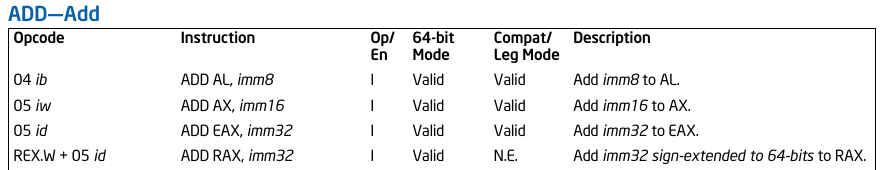
\includegraphics[width=6.5in]{pic/21a.png}
\\
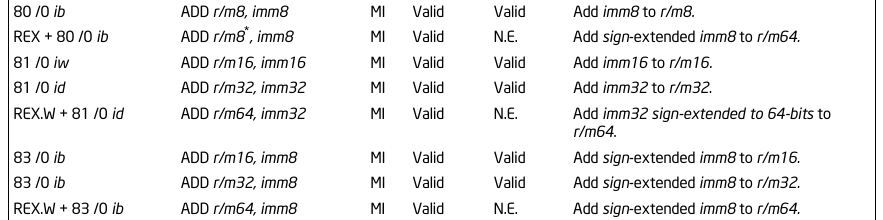
\includegraphics[width=6.5in]{pic/21b.png}
\\
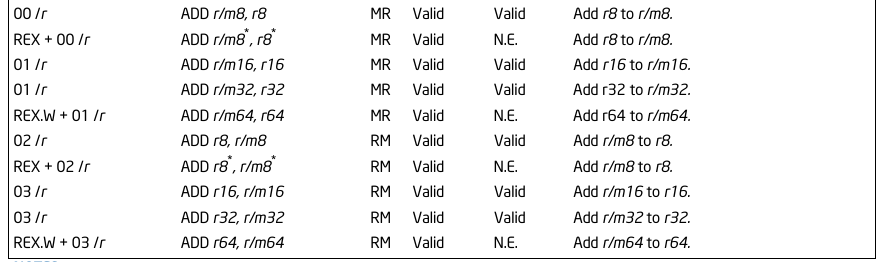
\includegraphics[width=6.5in]{pic/21c.png}
\\ \\
О-хо-хо! На одно только описание команды \texttt{ADD} ушла целая страница.
Что мы здесь видим?
\\ \\
Команда \texttt{ADD} описывается таблицей. Строки таблицы --- это разные варианты команды.
Колонки отвечают за разные характеристики команды:
``Opcode'' --- схема кодирования команды,
``Instruction'' --- общий вид команды,
``Op/En'' (Operand Encoding) --- тип кодирования операндов,
``64 Bit Mode'' и ``Compat/Leg Mode'' (Compatibility/Legacy Mode) --- работает ли команда в этих режимах процессора
(если помнишь, у процессоров x86 есть разные режимы),
``Description'' --- описание команды на человеческом языке.
\\ \\
У команды \texttt{ADD} есть четыре основных варианта, различающихся по типу операндов.
Это хорошо видно в колонке ``Op/En'': там встречаются четыре разных значения
I (immediate), MI (register/memory - immediate), RM (register - register/memory), MR (register/memory - register).
Каждый из этих четырёх вариантов дальше разветвляется по размеру операндов.
\\ \\
Какой вариант подходит нам?
В нашей программе числа 1 и 2 --- это константы (immediate operand).
Мы договорились, что компилятор работает с 32-битными числами, поэтому это 32-битные константы.
(Из таблицы должно быть понятнее, почему я выбрала 32, а не 64 бита: для 64-битных команд впереди добавляется некий REX-префикс, с которым возиться неохота.)
Нам подошла бы команда \texttt{ADD imm32, imm32}, но такой нет.
Зато есть очень похожие команды \texttt{ADD EAX, imm32} и \texttt{ADD r/m32, imm32}.
Команда \texttt{ADD EAX, imm32} берёт первое слагаемое из регистра EAX.
Команда \texttt{ADD r/m32, imm32} берёт первое слагаемое из любого регистра общего назначения или из памяти.
Понятно, что обе команды не идеальны: всё равно придётся загрузить первое слагаемое в память или в регистр.
Для этого нам понадобится другая команда --- \texttt{MOV}:
\\ \\
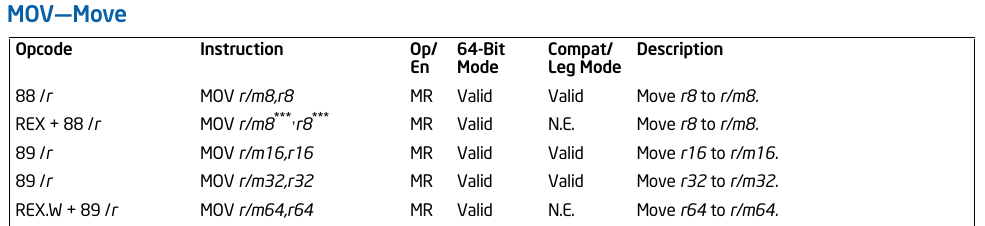
\includegraphics[width=6.5in]{pic/mov_1.png}
\\
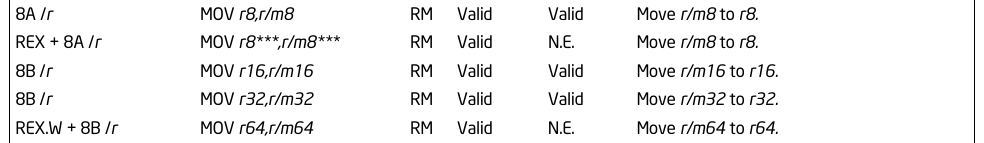
\includegraphics[width=6.5in]{pic/mov_2.png}
\\
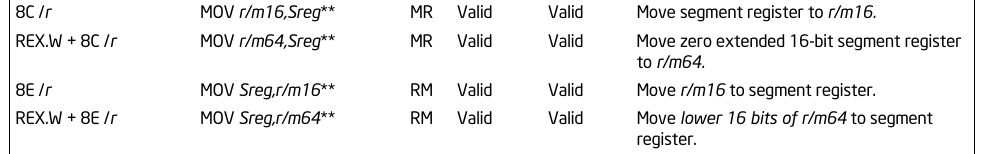
\includegraphics[width=6.5in]{pic/mov_3.png}
\\
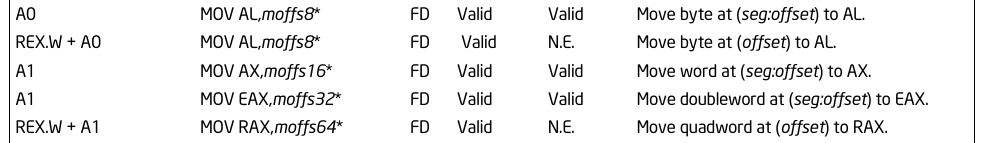
\includegraphics[width=6.5in]{pic/mov_4.png}
\\
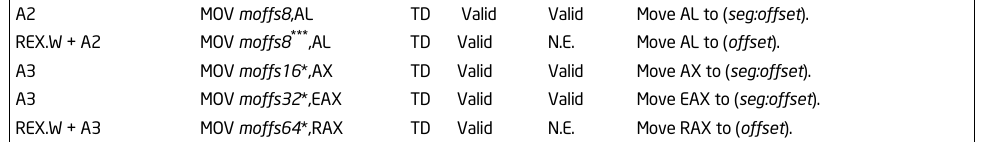
\includegraphics[width=6.5in]{pic/mov_5.png}
\\
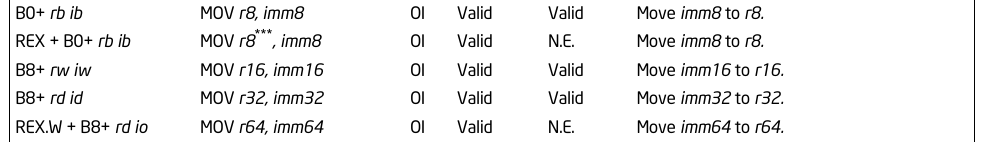
\includegraphics[width=6.5in]{pic/mov_6.png}
\\
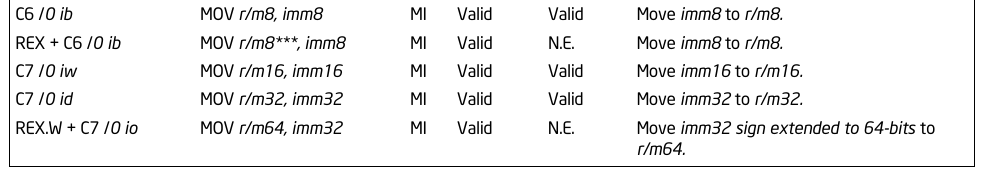
\includegraphics[width=6.5in]{pic/mov_7.png}
\\ \\
Час от часу не легче: вариантов ещё больше, чем у команды \texttt{ADD}.
И это только \texttt{MOV} для регистров общего назначения, а есть ещё \texttt{MOV}ы для другигих групп регистров.
Режимов кодирования операндов тоже прибавилось: кроме уже известных MI, RM и MR появились ещё FD, TD и OI.
Нам подходят варианты \texttt{MOV r32, imm32} и \texttt{MOV r/m32, imm32}.
\\ \\
Пора определиться: в регистр или в память мы будем записывать первое слагаемое,
и если в регистр, то в EAX или нет (команда \texttt{ADD} предусматривает отдельный вариант для EAX).
В архитектуре x86 часто возникают такие ситуации, когда одно и то же можно сделать несколькими разными способами.
Хороший компилятор старается всегда выбирать самый быстрый вариант.
В нашем случае, во-первых, регистры быстрее памяти --- поэтму следует хранить первое слагаемое в регистре.
Во-вторых, команда \texttt{ADD} явно оптимизирована для регистра EAX, поэтому следует хранить первое слагаемое в регистре EAX.
С учётом этого у нас получается такая ассемблерная программа:
\begin{verbatim}
    mov eax, 1
    add eax, 2
\end{verbatim}
Неплохо! Осталось перевести эту программу в машинные коды, то есть ассемблировать.
Как это сделать?
Самый правильный (но не самый простой) способ --- прибегнуть к старому другу, интеловскому мануалу.
Там подробно объясняется кодирование всех команд.
Я разберу только две команды из нашего примера --- полную схему кодирования ты всегда найдёшь в мануале.
\\ \\
Начнём с команды \texttt{mov eax, 1}.
В таблице ей соответствует вариант:
\\
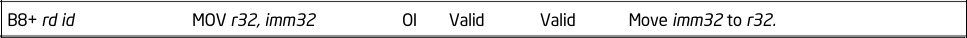
\includegraphics[width=6.5in]{pic/mov_r32_imm32.png}
\\
В первой колонке указана схема кодирования: \texttt{B8 + rd id}.
В мануале ``Intel 64 and IA-32 Architectures Software Developer's Manual'', том 2, глава 3.1.1, поясняются эти обозначения:
\begin{itemize}
\item \texttt{B8} --- однобайтный шестнадцатеричный опкод.
\item \texttt{rd} (register dword) --- однобайтный номер регистра.
Регистру EAX соответствует номер 0, поэтому байт равен \texttt{0x00}.
\item \texttt{B8 + rd} означает, что эти два байта надо сложить: \texttt{0xB8 + 0x00 = 0xB8}.
\item \texttt{id} (immediate dword) --- это 4-байтный непосредственный операнд.
У нас непосредственный операнд --- это константа 1, в шестнадцатеричном представлении --- \texttt{0x1}.
На её кодирование отводится целых четыре байта, в то время как сама константа занимает один бит.
Все остальные биты придётся забить нулями: \texttt{0x00 0x00 0x00 0x01}.
Это кажется напрасной тратой битов, но ведь вместо 1 могло бы быть любое число в диапазоне $[-2^{N - 1}, 2^{N - 1} - 1]$.
\end{itemize}
Итого, получаем команду --- \texttt{0xB8 0x00 0x00 0x00 0x01}, так?
\\ \\
Так, да не совсем.
Есть одна гадкая мелочь: почему мы решили, что 4-байтное число 1 должно кодироваться именно как \texttt{0x00 0x00 0x00 0x01}?
Потому что это \emph{естественно}: мы привыкли представлять числа от старших разрядов к младшим.
Однако число ничуть не изменится, если его представлять как-то по-другому: например, от младших разрядов к старшим.
Это дело договорённости: важно, чтобы все понимали представление одинаково.
Так вот архитектура x86 представляет себе числа от младших \emph{байтов} к старшим:
например, 4-байтное число \texttt{0x0A0B0C0D} предсталено в виде \texttt{0x0D 0x0C 0x0B 0x0A}.
Такой порядок байт называется \emph{little-endian}.
Другой порядок --- \emph{big-endian}, в нём байты хранятся от старших к младшим: \texttt{0x0A}, \texttt{0x0B}, \texttt{0x0C}, \texttt{0x0D}.
Само понятие порядка байт называется \textbf{endianness}.
\\
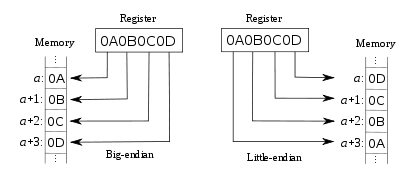
\includegraphics[height=1.75in]{pic/22.png}
\\
Исправленная команда выглядит так: \texttt{0xB8 0x01 0x00 0x00 0x00}.
\\
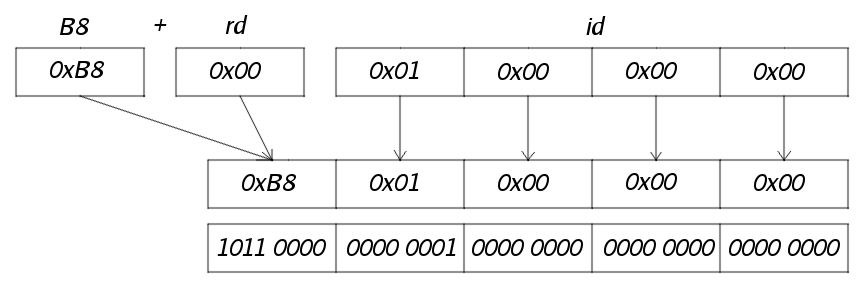
\includegraphics[height=1.25in]{pic/mov_eax_1.png}
\\ \\
Теперь ассемблируем вторую команду: \texttt{add eax, 2}.
Мы решили использовать вариант:
\\
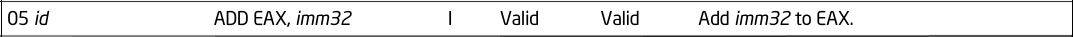
\includegraphics[width=6.5in]{pic/add_eax_imm32.png}
\\
На сей раз схема кодирования совсем простая: \texttt{05 id}.
Понятное дело, \texttt{05} --- однобайтный шестнадцатеричный опкод,
а \texttt{id} --- 4-байтный непосредственный операнд в форме little-endian.
Итого получаем команду \texttt{0x05 0x02 0x00 0x00 0x00}:
\\
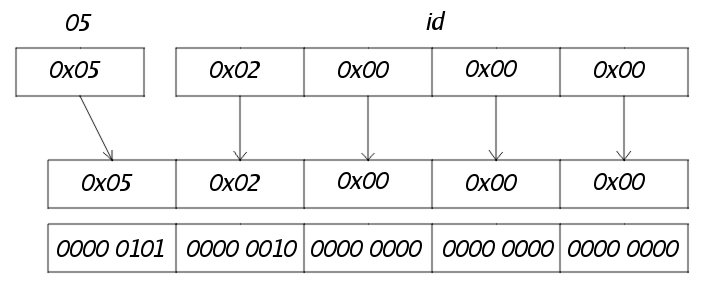
\includegraphics[height=1.25in]{pic/add_eax_2.png}
\\ \\
Объединяя обе команды, получаем итоговую программу: \texttt{0xB8 0x01 0x00 0x00 0x00 0x05 0x02 0x00 0x00 0x00}.
\\ \\
На самом деле можно было получить её гораздо проще с помощью какого-нибудь готового ассемблера.
(Здесь я понимаю ассемблер как программу, а не как язык.)
Синтаксис разных ассемблеров немного отличается.
Для ассемблера \texttt{nasm} исходная программа выглядит так (файл example.asm):
\lstinputlisting{nasm/example.asm}
Пришлось добавить директиву \texttt{BITS 64} --- она указывает ассемблеру, для какого режима процессора ассемблировать программу.
Ассемблируем:
\begin{verbatim}
$ nasm -O0 example.asm
\end{verbatim}
Флаг -O0 (нулевые оптимизации) заставляет \texttt{nasm} сохранять исходные команды
(по умолчанию \texttt{nasm} подыскивает более короткие эквивалентные команды).
Содежимое бинарного файла example можно посмотреть с помощью \texttt{mc}, открыв файл по \texttt{F3} и затем нажав \texttt{F4}:
\begin{verbatim}
0xB8 0x01 0x00 0x00 0x00 0x05 0x02 0x00 0x00 0x00
\end{verbatim}
Это полностью совпадает с тем, что мы наассемблировали руками.
Теперь можно из любопытства опустить флаг -O0:
\begin{verbatim}
$ nasm example.asm
\end{verbatim}
Первая команда (\texttt{mov eax, 1}) осталась неизменной, а вот вторую команду (\texttt{add eax, 2})
\texttt{nasm} оптимизировал: он заменил её более короткой командой \texttt{add r/m32, imm8}
(воспользовавшись тем, что константа 2 влазит в один байт):
\begin{verbatim}
0xB8 0x01 0x00 0x00 0x00 0x83 0xC0 0x02
\end{verbatim}
(Команда \texttt{add r/m32, imm8} узнаётся по опкоду \texttt{0x83} из таблицы для команды \texttt{ADD}).
Вот так мы узнали, что оказывается можно было составить более эффективную программу.
\\ \\
Дальше я не буду останавливаться на кодировании команд.
Некоторые команды кодируются намного хитрее, чем те, что мы видели,
особенно команды, работающие с памятью: у них есть сложные режимы адресации.
В нашем компиляторе будут использоваться в основном простые команды.
Это не всегда будут самые эффективные команды, но я и не замахивалась на оптимизирующий компилятор ---
понятно, что исходный язык настолько прост, что позволяет любую программу вычислить на этапе компиляции
(программы не зависят ни от каких внешних данных).
\\ \\
Ну что ж, побаловались с маленькой программой, пора переходить к компиляции принципиально \emph{любой} программы.
Чтобы не погибнуть в мутных примерах и частных случаях, понадобятся радикальные меры. :D
\\ \\
Как говорится, ``воспользуемся методом математической индукции''.
Программа представлена в виде AST, и индукцию мы будем проводить по высоте этого AST.
Листьями AST являются числа, узлами --- арифметические операции.
Сначала мы рассмотрим AST нулевой высоты: лист, и покажем, как его скомпилировать --- это будет база индукции.
Затем мы предположим, что любой AST высоты не более $k$ скомпилирован, и покажем, как на его основе скомпилировать любой AST высоты $k + 1$ --- шаг индукции.
Поехали!
\\ \\
Итак, база индукции: нужно скомпилировать лист AST, то есть константу $C$.
Нет ничего проще:
\begin{verbatim}
    mov eax, С
\end{verbatim}
Переходим к шагу индукции: нужно скомпилировать программу $p_1 \circ p_2$,
где $p_1$ и $p_2$ --- уже скомпилированные программы, а $\circ$ --- арифметическая операция.
Сразу возникает вопрос: где хранятся результаты выполнения программ $p_1$ и $p_2$?
Если $p_1$ --- лист, то результат $p_1$ хранится в регистре EAX.
Однако если $p_2$ --- тоже лист, то результат $p_2$ хранится тоже в регистре EAX!
Очевидно, если $p_2$ выполняется после $p_1$, то $p_2$ затрёт результат $p_1$:
\begin{verbatim}
    <p1>          ; result in EAX
    <p2>          ; result in EAX
    <op> eax, eax ; bad :(
\end{verbatim}
Что с этим делать?
Можно попытаться заставить разные подпрограммы использовать разные регистры:
например, пусть $p_1$ сохраняет результат в EAX, а $p_2$ --- в EBX:
\begin{verbatim}
    <p1>          ; result in EAX
    <p2>          ; result in EBX
    <op> eax, ebx ; result in EAX
\end{verbatim}
Всё хорошо, пока не задумываешься, что из себя представляют $p_1$ и $p_2$.
Это ведь \emph{любые} программы, они могут быть очень большими и ветвиться на сколько угодно подпрограмм.
Все эти подпрограммы как-то делят между собой регистры.
Что если подпрограмм больше, чем регистров?
Например, если $p_1 = C_1 + (C_2 + (... + (C_{N - 1} + C_N)...))$, то по нашей логике программа для $p_1$ должна скомпилироваться так:
\begin{verbatim}
    mov r1, C1         ; result in r1
    mov r2, C2         ; result in r2
    ...
    mov r(N-1), C(N-1) ; result in r(N-1)
    mov r(N), C(N)     ; result in r(N)
    add r(N-1), rN     ; result in r(N-1)
    ...
    add r1, r2         ; result in r1
\end{verbatim}
Ясно, что для больших $N$ регистров не хватит.
Есть и другая неприятность: запрет использования отдельных регистров вносит асимметрию.
Две одинаковых подпрограммы могут скомпилироваться по-разному только потому, что им будут доступны разные регистры.
Сама компиляция тоже усложняется: нужно постоянно следить за тем, какие регистры свободны.
Короче, ничё хорошего.
Явно регистрами тут не обойтись.
\\ \\
Очевидный выход --- сохранять результат программы $p_1$ в память.
(Результат программы $p_2$ сохранять не надо, он сразу же используется.)
На вопрос ``а если памяти не хватит?'' я могу ответить только ``будет плохо!''.
На самом деле, если нам попадётся \emph{настолько} большая программа, проблемы начнутся гораздо раньше
и решать их придётся другими способами (разбивать программу на куски).
Нас эти проблемы не особо интересуют, поскольку они общие для большинства программ, а не специфичные для компилятора.
Будем считать, что памяти много.
\\ \\
Итак, сохраняем результат программы $p_1$ в память (допустим, у нас есть большой кусок памяти):
\begin{verbatim}
    <p1>
    mov [addr], eax ; result in [addr]
    <p2>            ; result in eax
    mov ebx, [addr]
    <op> eax, ebx   ; result in eax
\end{verbatim}
Эта схема вполне работоспособна и можно было бы на ней остановиться.
Но она, честно говоря, малось корявая.
Компилятору придётся много возиться с адресами:
программа $p_2$ может рекурсивно ветвиться на другие подпрограммы, которые тоже будут сохранять результат в память.
Компилятору придётся запоминать, где чей результат.
Хуже того: когда результат подпрограммы читается из памяти, он больше не нужен, и хорошо бы эту память использовать повторно.
Значит, компилятору придётся следить за тем, какие ячейки памяти свободны (ну или использовать память нерационально).
\\ \\
Этого всего можно избежать, если заметить, что в нашем случае порядок вычислений позволяет хранить значения в стеке.
\\
\bigskip
\begin{minipage}{0.6\textwidth}
Стек --- это кусок памяти, доступ к которому осуществляется с помощью команд \texttt{PUSH} и \texttt{POP}:
\texttt{PUSH} ``запихивает'' значение на вершину стека, а \texttt{POP} ``выпихивает'' последнее записанное значение.
Получается, что значения читаются в порядке, обратном порядку записи.
Указатель на вершину стека храниться в регистре ESP (Stack Pointer), и команды \texttt{PUSH} и \texttt{POP} сами обновляют его:
\texttt{PUSH} уменьшает ESP на размер операнда и записывает операнд в память по адресу [ESP],
а \texttt{POP} читает значение из памяти по адресу [ESP] в операнд и увеличивает ESP на размер операнда.
\end{minipage}
\begin{minipage}{0.4\textwidth}
\centering
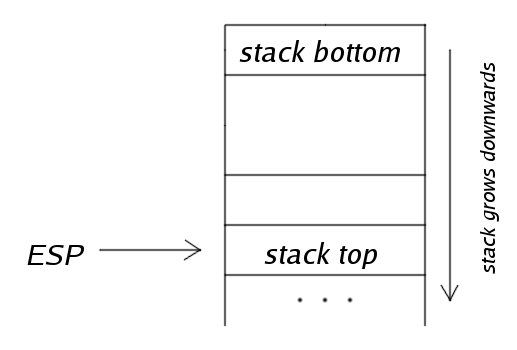
\includegraphics[width=\textwidth]{pic/stack.png}
\end{minipage}
\bigskip
\\
Казалось бы, довольно специфичная структура --- но стек оказывается полезен во многих задачах.
Он позволяет работать со вложенными (древовидными) структурами:
узел-потомок начинает обрабатывться позже, чем узел-предок, а заканчивает раньше
(что соответствует принципу LIFO).
Если бы AST представляло из себя не дерево, а произвольный граф, то стеком мы бы не отделались.
\\ \\
С учётом стека произвольный узел AST вида $p_1 \circ p_2$ компилируется так:
\begin{verbatim}
    <p1>
    push eax
    <p2>
    pop ebx
    <op> eax, ebx ; result in eax
\end{verbatim}
Это уже очень хороший и почти окончательный вариант. :)
Осталось подправить две мелочи, связанные с кодированием команд.
\\ \\
Первая мелочь касается неразберихи с битностью, командами и режимами процессора.
Мы нигде явно не договаривались, для какого режима процессора мы компилируем программы.
Помнится, я сказала, что мы будем использовать 32-битную, а не 64-битную арифметику, потому что она проще кодируется.
Значит ли это, что мы автоматически выбрали 32-битный режим?
Нет.
Команды 32-битной арифметики доступны в обоих режимах (это написано в их таблицах в колонках ``64 Bit Mode'' и ``Compat/Leg Mode'').
Давай определимся: пусть наши программы будут 64-битные --- как-никак мы компилируем для 64-битного процессора.
Это решение никак не повлияет на арифметические команды, но немного повлияет на команды \texttt{PUSH} и \texttt{POP}.
Как видно из таблицы для команды \texttt{PUSH}, в 64-битном режиме нет команды \texttt{PUSH r/m32} --- есть только команда \texttt{PUSH r/m64}.
Эти две команды кодируются абсолютно одинаково --- строго говоря, это одна команда, интерпретация которой зависит от режима.
Аналогично с командой \texttt{POP}.
Исправленная программа выглядит так:
\begin{verbatim}
    <p1>
    push rax
    <p2>
    pop rbx
    <op> eax, ebx ; result in eax
\end{verbatim}
Может показаться, что нельзя так перемешивать 32-битные и 64-битные регистры,
но заметь, что в вычислениях участвуют только 32-битные регистры, а их старшие половины просто занимают лишнее место в стеке.
\\ \\
Вторая мелочь связана с кодированием арифметических команд.
У нас первый операнд находится в регистре EBX, а второй --- в регистре EAX.
Результат мы хотим получить в регистре EAX.
Со сложением всё хорошо: есть команда \texttt{add eax, ebx}, котоая прибавляет EBX к EAX.
С умножением тоже всё хорошо: команда \texttt{imul ebx} умножает EAX на EBX.
Из-за коммутативности сложения и умножения нам безразличен порядок операндов.
С вычитанием всё хуже: команда \texttt{sub eax, ebx} вычитает EВX из EAX (перепутаны уменьшаемое и вычитаемое),
а команда \texttt{sub ebx, eax} делает что надо, но записывает результат в EBX ---
значит, придётся менять операнды местами или перемещать результат.
С делением совсем плохо: делимое обязательно должно быть в регистре EAX (других вариантов просто нет).
Очевидное решение --- поменять операнды местами (для этого есть даже специальная команда \texttt{XCHG}).
Но есть более элегантное решение: можно поменять местами подпрограммы $p_1$ и $p_2$:
\begin{verbatim}
    <p2>
    push rax
    <p1>
    pop rbx
    <op> eax, ebx ; result in eax
\end{verbatim}
Наконец, есть ещё одна мелочь:
произведение двух 32-битных чисел может быть 64-битным числом, поэтому команда \texttt{IMUL}
записывает результат не просто в EAX, а в пару регситров EDX:EAX.
Мы работаем с 32-битными числами и игнорируем старшую часть результата: что не влезло, то не влезло.
Но с командой \texttt{IDIV} просто проигнорировать не получится: она берёт старшую часть делимого из регистра EDX,
поэтому если там будет мусор, результат деления будет неправильным.
Перед делением мы должны заполнить регистр EDX старшим (знаковым) битом делимого (sign-extend EDX of EAX): если делимое положительное, EDX = 0,
если отрицательное --- EDX = 0xFFFFffff.
В этом нам поможет команда \texttt{CDQ} (Convert Double to Quad).
(Если непонятно, почитай про двоичное представление отрицательных чисел в виде дополнения до двух: two's complement.)
\\ \\
Окончательный алгоритм компиляции AST в код для x86-64 выглядит так:
\begin{verbatim}
compile(p):
    if p = C:
        mov eax, C
    else if p = p1 + p2:
        compile(p2)
        push rax
        compile(p1)
        pop rbx
        add eax, ebx
    else if p = p1 - p2:
        compile(p2)
        push rax
        compile(p1)
        pop rbx
        sub eax, ebx
    else if p = p1 * p2:
        compile(p2)
        push rax
        compile(p1)
        pop rbx
        imul ebx
    else if p = p1 / p2:
        compile(p2)
        push rax
        compile(p1)
        pop rbx
        cdq
        idiv ebx
\end{verbatim}
Всё!
С генерацией кода разобрались. :)
Вот кусок компилятора, который генерирует код по AST:
\lstinputlisting[language=C++]{example_lang_proc/compiler.cpp}
Компилятор, как и интерпретатор, рекурсивно обходит AST,
только вместо немедленных вычислений он генерирует машинные инструкции и сохраняют их в массив байтов.
Компиляцию операндов я вынесла в отдельную функцию, потому что она везде повторяется.
\\ \\
Вообще говоря, на этом задача компилятора выполнена: мы разобрались с архитектурой x86 и научлились компилировать AST в машинный код.
Но для души этого мало: надо ещё запустить скомпилированную непосильным тудом программу на настоящем процессоре.
(Как минимум, проверить, что она работает. :D)
\\ \\
Обычно компилятор сохраняет скомпилированную программу в виде объектного файла.
Объектный файл содержит машинный код и разную информацию: статические данные,
таблицу симовлов (экспортируемые и импортируемые функции, глобальные переменные и т.д.),
релокации (адреса в программе надо настраивать в соответствии с адресом, по которому программа будет загружена в память),
информацию для дебага и прочее.
Когда компилятор скомпилировал все единицы трансляции в объектные файлы, наступает черёд линкера.
Линкер связывает все объектные файлы в один исполняемый файл: настраивает релокации, разрешает зависимости и т.д.
Линковка --- отдельная тема, сложная и интересная, и я не буду её трогать.
Нам линкер не нужен --- наши программы всегда состоят из одной самодостаточной единицы трансляции и не возятся с адресами в памяти.
Мы можем сразу же сохранять программу в виде исполняемого файла.
\\ \\
Формат исполняемых файлов специфичен для операционной системы.
В линуксе принят формат ELF (Executable and Linkable Format), и мы рассмотрим его 64-битную версию: ELF-64.
Описание этого формата ты можешь найти в \texttt{man elf} (или в интернедах).
\\ \\
\begin{minipage}{0.5\textwidth}
ELF-файл предназначен для хранения двух типов файлов: объектных (relocatable) и исполняемых (loadable).
С объектными файлами работает линкер, с исполняемыми --- загрузчик.
\\ \\
Любой ELF-файл начинается с ELF-заголовка, который
описывает ключевые характеристики файла и взаимное расположение остальных частей файла:
таблицы программных заголовков, таблицы разделов и самих сегментов или разделов.
Таблица программных заголовков необязательна для объектных файлов, а таблица разделов необязательна для исполняемых файлов.
\end{minipage}
\begin{minipage}{0.5\textwidth}
\centering
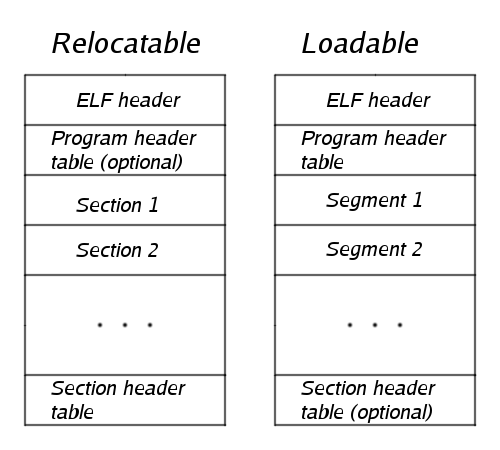
\includegraphics[width=\textwidth]{pic/elf.png}
\end{minipage}
\\ \\
\begin{minipage}{0.75\textwidth}
Наши ELF-файлы будут состоять из трёх частей:
\begin{enumerate}
\item ELF-заголовок.
\item Таблица программных заголовков с единственным заголовком, описывающим сегмент кода.
\item Сегмент кода, содержащий код программы.
\end{enumerate}
\end{minipage}
\begin{minipage}{0.25\textwidth}
\centering
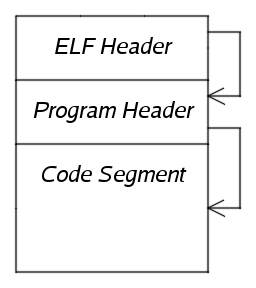
\includegraphics[width=\textwidth]{pic/elf2.png}
\end{minipage}
\\ \\
Как нам проще всего сгенерировать заголовки?
Можно руками записать нужные байты в файл, пользуясь спецификацией и внимательно следя за размером и содержимым каждого поля.
Но в линуксе есть С-шный заголовочный файл ``elf.h'', в котором определены структуры заголовков и много удобных макросов и констант с красивыми названиями.
Использование этого хедера сделает наш компилятор непортабельным:
компилятор невозможно будет собрать в другой операционной системе, где нет такого хедера.
Но честно говоря, наш компилятор и так не отличается особой портабельностью:
генерирует код для специфичной архитектуры x86\_64 и сохраняет его в специфичном формате ELF-64.
\\ \\
ELF-заголовок состоит из следующих полей:
\\ \\
\begin{minipage}{0.5\textwidth}
\begin{itemize}
\item Группа полей ``ELF Identification'':
    \begin{itemize}
    \item Четырёхбайтовая сигнатура \texttt{0x7f 0x45 0x4c 0x46} (``magic'').
    Если ты откроешь в \texttt{mc} по Shift+F3 какой-нибудь ELF-файл, ты увидишь эту сигнатуру: первый символ (\texttt{0x7f}) непечатный, а остальные три
    (\texttt{0x45 0x4c 0x46}) образуют слово ``ELF''.
    Наличие уникальной сигнатуры характерно для бинарных форматов.
    \item Класс (разрядность): у нас ELFCLASS64.
    \item Кодирование данных: у нас ELFDATA2LSB.
    \item Номер версии формата ELF:у нас EV\_CURRENT.
    \item OS ABI (Operation System Application Binary Interface, бинарный интерфейс операционной системы): у нас, видимо, ELFOSABI\_LINUX.
    \item Номер версии OS ABI: в \texttt{man elf} советуют 0.
    \item Семь зарезервированных байтов (нулевых).
    \end{itemize}
\item Тип: у нас ET\_EXEC (исполняемый).
\item Архитектура: у нас EM\_X86\_64.
\item Номер версии файла: у нас, видимо, EV\_CURRENT.
\item Точка входа (адрес в памяти, на который загрузчик передаст управление): пока непонятно, откуда его взять.
\item Смещение таблицы программных заголовков: у нас она идёт сразу после ELF-заголовка, поэтому смещение равно размеру ELF-заголовка.
\end{itemize}
\end{minipage}
\begin{minipage}{0.5\textwidth}
\centering
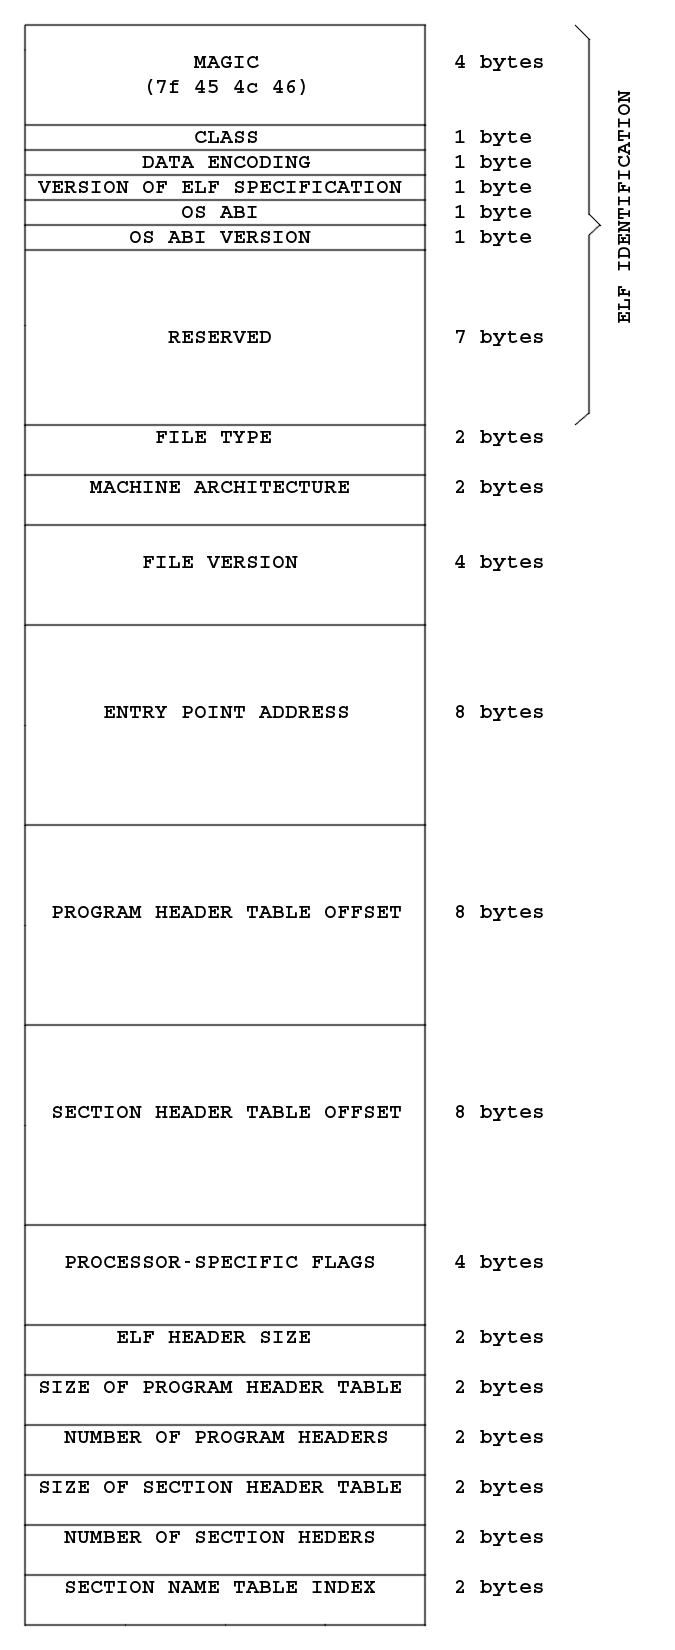
\includegraphics[width=\textwidth]{pic/elf_header.png}
\end{minipage}
\begin{itemize}
\item Смещение таблицы разделов: в \texttt{man elf} говорят, что если этой таблицы нету, то смещение 0.
\item Процессоро-специфичные флаги: в \texttt{man elf} советуют 0.
\item Размер ELF-заголовка: фиксирован, можно посчитать (но в С есть удобный оператор \texttt{sizeof}, позволяющий получить размер структуры).
\item Размер таблицы программных заголовков: равен размеру программного заголовка (у нас всего один заголовок в таблице).
\item Число программных заголовков: у нас 1.
\item Размер таблицы разделов: у нас её нет, поэтому 0.
\item Число разделов: 0.
\item Номер раздела, содержащего таблицу имён разделов: у нас такого раздела нет, поэтому SHN\_UNDEF.
\end{itemize}
Программный заголовок описывает сегмент (в нашем случае сегмент кода) и состоит из следующих полей:
\\ \\
\begin{minipage}{0.65\textwidth}
\begin{itemize}
\item Тип сегмента: у нас PT\_LOAD (загрузочный).
\item Атрибуты сегмента: у нас PF\_X и PF\_R (доступен на исполнение и чтение).
\item Смещение сегмента от начала файла (равно размеру ELF-заголовка).
\item Адрес загрузки сегмента в виртуальную память
(пока непонятно, откуда взять этот адрес).
\item Адрес загрузки сегмента в физическую память
(поле зарезервировано для систем, в которых напрямую адресуется физическая память, у нас должно быть нулевым).
\item Размер сегмента в файле (равен размеру кода).
\item Размер сегмента в памяти (равен размеру кода).
\item Выравнивание.
Обычно программа ничего не знает о том, в какой области памяти располагается её код и данные.
Но иногда при работе с памятью хочется иметь какие-то гарантии:
например, что адрес выделенного блока памяти достаточно ``круглый'',
то есть несколько его младших битов --- нули.
Это позволяет использовать младшие биты адреса для своих нужд
(поскольку адрес однозначно определяется старшими, ненулевыми битами).
Наша программа не делает никаких подобных предположений, поэтому выравнивание нам не критично --- сойдёт 0.
\end{itemize}
\end{minipage}
\begin{minipage}{0.35\textwidth}
\centering
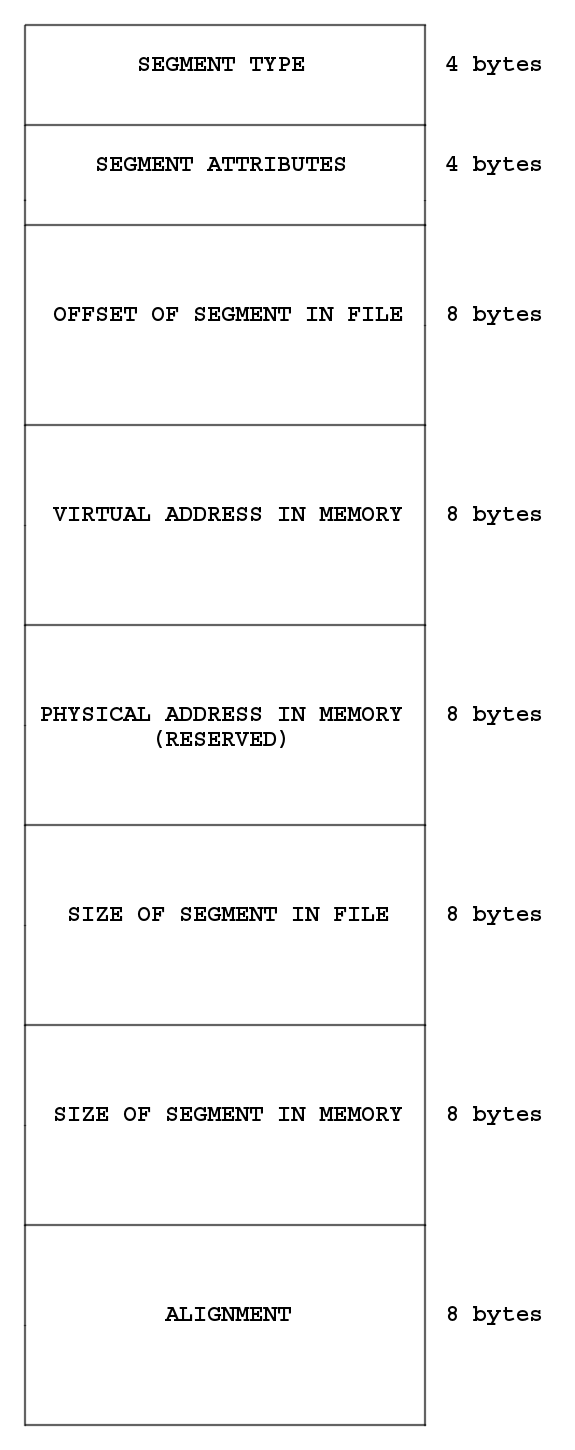
\includegraphics[width=\textwidth]{pic/elf_program_header.png}
\end{minipage}
\\ \\
Итак, осталось два непонятных поля: точка входа (из ELF-заголовка) и адрес загрузки сегмена кода в память (из программного заголовка).
В нашем случае оба поля совпадают: это адрес в памяти, на который загрузчик передаст управление, когда загрузит программу в память.
Но откуда взять это адрес: может ли он быть любым, или нужен какой-то стандартный?
Если у двух программ этот адрес совпадёт, они что, загрузятся в одну и ту же область памяти?
Чтобы ответить на эти вопросы, надо представлять, как программы загружаются в память.
\\ \\
\begin{minipage}{0.5\textwidth}
На файловой системе программа хранится в виде исполняемого файла (например, в формате ELF).
Это очень компактное представление: собственно код программы, инициализированные статические данные (у нас их нет) и вспомогательная информация.
\\ \\
Чтобы исполнить программу, загрузчик разворачивает её из компактного представления в \emph{образ} в памяти:
к коду и статическим данным добавляются стек и куча --- области памяти, в которых программа будет сохранять данные по мере исполнения.
\end{minipage}
\begin{minipage}{0.5\textwidth}
\centering
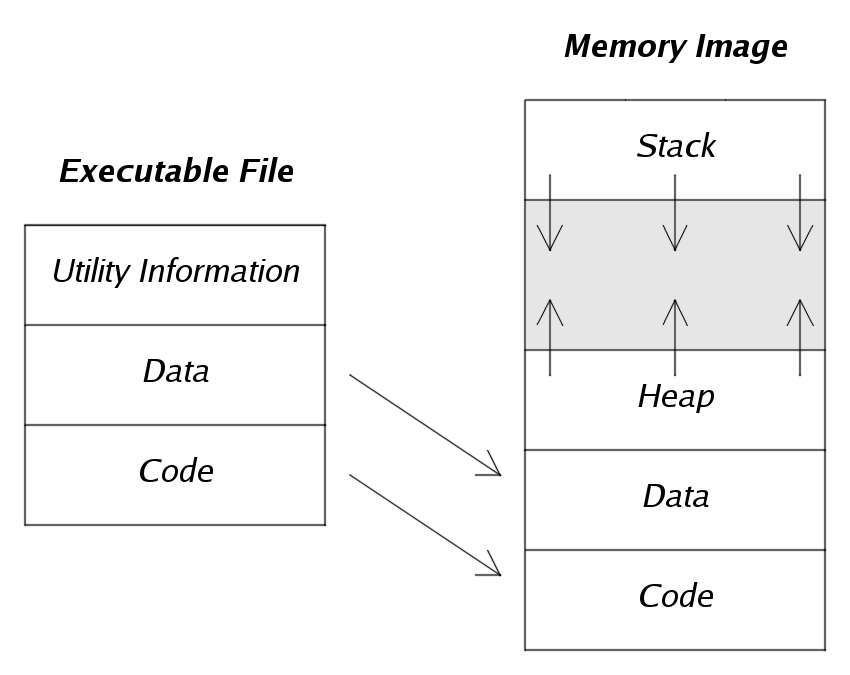
\includegraphics[width=\textwidth]{pic/executable_image.png}
\end{minipage}
\\ \\
Размер стека и кучи не фиксирован (во время исполнения программа может выделять и освобождать память),
поэтому стек располагается в старших адресах памяти и растёт вниз,
а куча располагается в младших адресах (сразу после кода и даных) и растёт вверх.
При таком раскладе возникают два вопроса:
\begin{enumerate}
\item Что если одни части программы налезут на другие (например, стек на кучу)?
\item Что если надо одновременно загрузить в память несколько программ, как поделить память между ними?
\end{enumerate}
На оба эти вопроса ответ один --- виртуальная память.
\\ \\
Я уже немного рассказывала про виртуальную память: это логическое представление оперативной памяти
(обычно поверх другого логического представления --- сегментной модели памяти).
Каждой программе память представлется в виде виртуального адресного пространства.
В этом виртуальном адресном пространстве нет других программ (кроме ядра операционной системы и, возможно, динамических библиотек):
программе надо неслабо постараться, чтоб влезть в чужое адресное пространство.
Размер виртуального адресного пространства зависит от разрядности адреса: $2^N$ для архитектуры с N-битными адресами,
то есть 4 гигабайта для 32-битных адресов и 2 эксабайта для 64-битных адресов.
В архитектуре x86\_64 размер виртуального адресного пространства --- 256 терабайт (не все 64 бита адреса используются).
Это значительно превышает объём физической оперативной памяти (обычно несколько гигабайт).
\\ \\
Виртуальная память реализована на основе страничного механизма процессора:
адресное пространство разбито на страницы, которые по мере надобности загружаются в физическую память и выгружаются из неё.
Операционная система настраивает процессор и следит за отображением виртуальных страниц на физическую память.
Часть страниц виртуальной памяти привязана к реальной (оперативной или внешней) памяти (mapped), другие не привязаны (unmapped).
У каждой страницы есть права доступа на запись/чтение/исполнение (unmapped страницы недоступны ни на что).
Всё управление виртуальной памятью (выделение/освобождение/изменение прав доступа) программа вынуждена делать через операционую систему.
Если программа попытается нарушить права доступа к странице, операционная система поймает это нарушение и прервёт исполнение программы.
\\ \\
\begin{minipage}{0.35\textwidth}
Виртуальная память решает сразу несколько проблем.
Во-первых, разные части программы не налезут друг на друга: в виртуальном адресном пространстве между ними находятся ``буферные'' страницы (unmapped),
доступ к которым запрещён.
Во-вторых, загрузить несколько программ в память тоже не проблема: операционная система просто должна распределять
физическую память сразу между несколькими виртуальными пространствами.
При этом разные программы изолированы друг от друга.
В-третьих, для самих программ управление памятью значительно упрощается.
Из недостатков --- доступ к памяти становится ещё медленнее (особенно с учётом page fault'ов).
\end{minipage}
\begin{minipage}{0.65\textwidth}
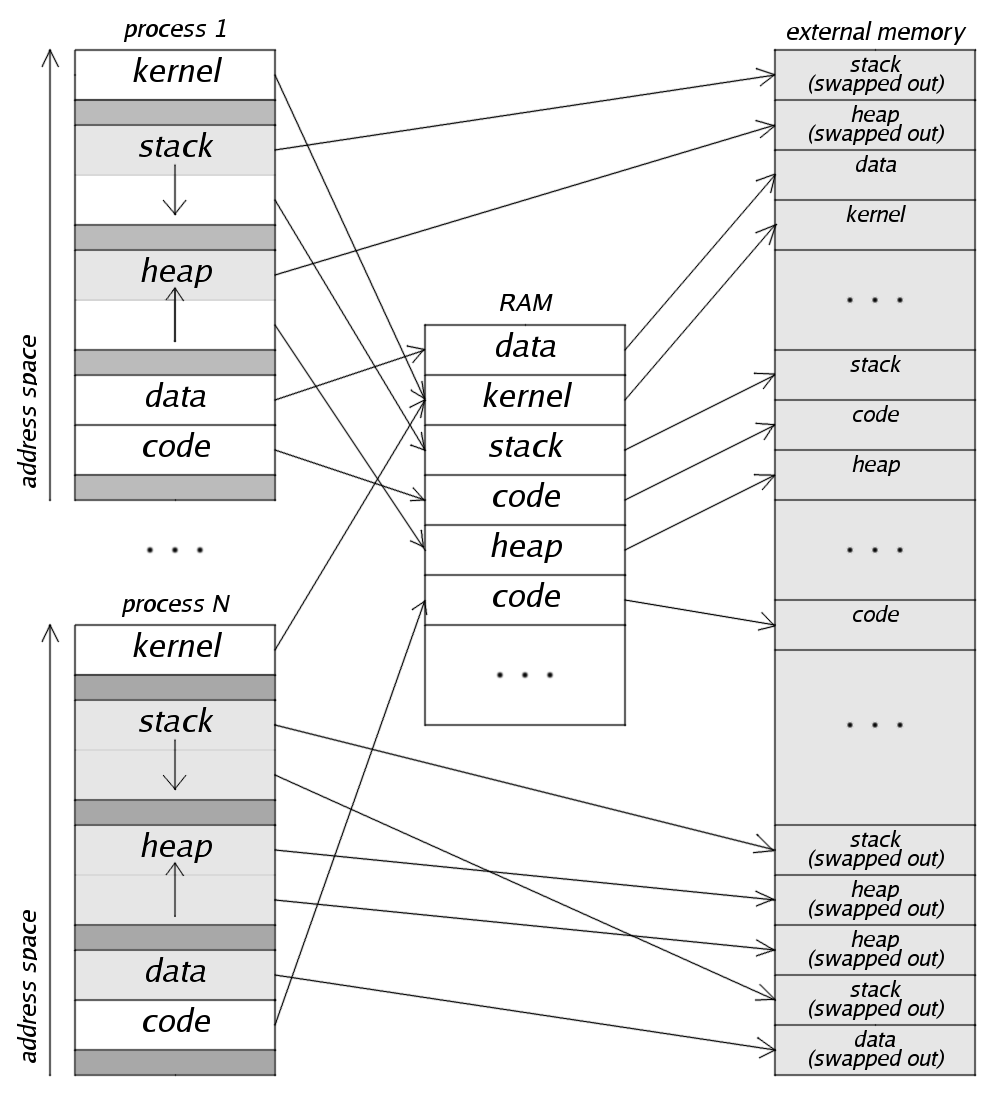
\includegraphics[width=\textwidth]{pic/virtual_memory.png}
\end{minipage}
\\ \\
Я уже говорила (и нарисовала на картинке), что в адресном пространстве любой программы присутствует ядро операционной системы.
Зачем?
Во-первых, полезная программа не может без операционной системы:
выделение памяти, работа с файлами, межпроцессные взаимодействия --- всё требует системных вызовов.
Во-вторых, даже если сама программа не взаимодействует с операционной системой,
операционной системе может понадобиться провзаимодействовать с программой (напрмер, прервать её выполнение).
В-третьих, ядро операционной системы всё равно должно быть загружено в физическую память
(операционная система исполняется дольше всех программ, которые запущены из неё),
поэтому ничего не стоит замапить его в виртуальную память любой программы.
\\ \\
Кроме ядра операционной системы, программы часто используют библиотеки.
Следует различать \emph{статические} и \emph{динамические} библиотеки:
статические зашиваются прямо в программу (линкером),
а динамические отдельно грузятся в адресное пространство программы
(загрузчиком или самой программой во время исполнения).
Если программа написана на языке высокого уровня,
она почти наверняка будет слинкована со стандартной библиотекой этого языка.
\\ \\
Теперь можно вернуться к нашим недовычисленным полям: точке входа (\texttt{e\_entry}) и адресу загрузки сегмента кода (\texttt{p\_vaddr}).
Оба поля означают виртуальный адрес загрузки программы в память.
На этот адрес есть некоторые ограничения.
Первое ограничение --- по нулевому адресу грузить программу нельзя: там располагается одна из ``буферных'' областей виртуальной памяти.
Размер этой области в линуксе записан в файле /proc/sys/vm/mmap\_min\_addr.
Второе ограничение --- если внимательно прочитать \texttt{man elf}, то там написано, что \texttt{p\_vaddr} и \texttt{p\_offset}
должны быть сравнимы по модулю \texttt{p\_align} (давать одинаковый остаток от деления на \texttt{p\_align}).
С учётом обоих ограничений положим \texttt{e\_entry = p\_vaddr = mmap\_min\_addr + p\_offset}.
\\ \\
Ну что, всё? Почти. :)
Есть одна мелочь: наша программа не останавливается.
Скомпилировать-то мы её скомпилируем, потом загрузим в память и передадим на неё управление.
Программа радостно выполнится, и ...?
Никакой магии не произойдёт, начнут выполняться следующие за сегментом кода байты в памяти.
В лучшем случае эти байты окажутся в области памяти, недоступной на выполнение, и операционная система прибьёт программу сегфолтом.
В худшем случае может быть что угодно: начнёт исполняться неизвестный код
(который, может быть, только и ждал, пока какой-нибудь лапоть передаст на него управление).
\\ \\
Чтобы избежать этого позора, нам надо как-то завершить программу.
Вообще, это сделать довольно просто: достаточно вызвать какое-нибудь гадкое исключение.
Можно поделить на ноль,
можно обратиться по нулевому адресу,
можно попытаться исполнить невалидную команду процессора.
Во всех этих случаях операционная система гарантированно прибьёт программу (гарантированно --- это важно!).
Но есть способ завершить программу по-хорошему: сделать системный вызов \texttt{exit}.
Как видишь, даже наша простецкая программа не обошлась без системных вызовов.
\\ \\
В линуксе, чтобы сделать системный вызов, нужно положить номер вызова в EAX,
аргументы в другие регистры, и выполнить 80-е прерывание.
Номер \texttt{exit} --- 1, единственный аргумент --- код возврата в EBX.
Наша программа сохраняет результат выполнения в EAX, поэтому получаем такой код:
\begin{verbatim}
    mov ebx, eax
    mov eax, 1
    int 80
\end{verbatim}
Этот код должен идти сразу после кода программы.
Результат будет в коде возврата.
Посмотреть его можно командой \texttt{echo \$?}, выполнив её сразу после выполнения программы.
Правда, если результат не влазит в 1 байт, мы его не увидим:
старшие байты операционная система использует для своих нужд (выставляет там разные ошибки и статусы).
Кроме того, шелл может обрубить ещё половину кодов (сужая диапазон до $[0, 127]$).
Наконец, код возврата интерпретируется как беззнаковое число, поэтому отрицательные результаты мы тоже не увидим.
По-хорошему, нельзя возвращать 32-битный знаковый результат программы в коде возврата,
но в противном случае пришлось бы выводить результат на экран (конвертировать число в строку и делать системный вызов),
а я решила, что с тебя уже хватит. ;)
\\ \\
Вот теперь действительно всё.
Код генерации ELF-файла вот (файл gen\_elf64.h):
\lstinputlisting[language=C++]{example_lang_proc/gen_elf64.cpp}
А вот хедер компилятора (файл compiler.h):
\lstinputlisting[language=C++]{example_lang_proc/compiler.h}
Фух. Тяжёлая выдалась глава про компилятор.
Тут тебе и архитектура x86\_64 с её регистрами и набором команд,
и алгоритм компиляции AST в машинные инструкции, и формат ELF-64, и виртуальная память.
И главное, результат --- непортабельный компилятор для одной-единственной архитектуры.
В сравнении с полстраницей кода интерпретатора это как-то слишком.
Возникает вопрос: это всегда так просто писать интерпретаторы и так тяжело --- компиляторы?
Ответ --- в общем, да.
В компиляторе добавляется серьёзный этап --- генерация кода (причём хороший компилятор умеет компилировать сразу под много архитектур).
Зато как это прекрасно --- машинные инструкции, и всё такое. :D
\\ \\
Кроме того, помни, что в нашем примере полностью отсутствует оптимизация промежуточного представления.
С учётом оптимизаций разница в сложности компилятора и интерпретатора была бы не такой разительной.

\section{Виртуальная машина: байткод}
\lstinputlisting[language=C++]{example_lang_proc/vm_bytecode.cpp}
\lstinputlisting[language=C++]{example_lang_proc/vm_bytecode.h}
\section{Виртуальная машина: интерпретатор байткода}
\lstinputlisting[language=C++]{example_lang_proc/vm_run.cpp}
\lstinputlisting[language=C++]{example_lang_proc/vm_run.h}
\section{Виртуальная машина: JIT-компилятор байткода}
\lstinputlisting[language=C++]{example_lang_proc/vm_jit.cpp}
\lstinputlisting[language=C++]{example_lang_proc/vm_jit.h}

\end{document}